\PassOptionsToPackage{unicode=true}{hyperref} % options for packages loaded elsewhere
\PassOptionsToPackage{hyphens}{url}
%
\documentclass[]{article}
\usepackage{lmodern}
\usepackage{amssymb,amsmath}
\usepackage{ifxetex,ifluatex}
\usepackage{fixltx2e} % provides \textsubscript
\ifnum 0\ifxetex 1\fi\ifluatex 1\fi=0 % if pdftex
  \usepackage[T1]{fontenc}
  \usepackage[utf8]{inputenc}
  \usepackage{textcomp} % provides euro and other symbols
\else % if luatex or xelatex
  \usepackage{unicode-math}
  \defaultfontfeatures{Ligatures=TeX,Scale=MatchLowercase}
\fi
% use upquote if available, for straight quotes in verbatim environments
\IfFileExists{upquote.sty}{\usepackage{upquote}}{}
% use microtype if available
\IfFileExists{microtype.sty}{%
\usepackage[]{microtype}
\UseMicrotypeSet[protrusion]{basicmath} % disable protrusion for tt fonts
}{}
\IfFileExists{parskip.sty}{%
\usepackage{parskip}
}{% else
\setlength{\parindent}{0pt}
\setlength{\parskip}{6pt plus 2pt minus 1pt}
}
\usepackage{hyperref}
\hypersetup{
            pdftitle={Is there a trade-off between compactness and communities of interest?},
            pdfborder={0 0 0},
            breaklinks=true}
\urlstyle{same}  % don't use monospace font for urls
\usepackage{graphicx,grffile}
\makeatletter
\def\maxwidth{\ifdim\Gin@nat@width>\linewidth\linewidth\else\Gin@nat@width\fi}
\def\maxheight{\ifdim\Gin@nat@height>\textheight\textheight\else\Gin@nat@height\fi}
\makeatother
% Scale images if necessary, so that they will not overflow the page
% margins by default, and it is still possible to overwrite the defaults
% using explicit options in \includegraphics[width, height, ...]{}
\setkeys{Gin}{width=\maxwidth,height=\maxheight,keepaspectratio}
\setlength{\emergencystretch}{3em}  % prevent overfull lines
\providecommand{\tightlist}{%
  \setlength{\itemsep}{0pt}\setlength{\parskip}{0pt}}
\setcounter{secnumdepth}{5}
% Redefines (sub)paragraphs to behave more like sections
\ifx\paragraph\undefined\else
\let\oldparagraph\paragraph
\renewcommand{\paragraph}[1]{\oldparagraph{#1}\mbox{}}
\fi
\ifx\subparagraph\undefined\else
\let\oldsubparagraph\subparagraph
\renewcommand{\subparagraph}[1]{\oldsubparagraph{#1}\mbox{}}
\fi

% set default figure placement to htbp
\makeatletter
\def\fps@figure{htbp}
\makeatother

\usepackage{booktabs}
\usepackage[]{natbib}
\bibliographystyle{plainnat}

\title{Is there a trade-off between compactness and communities of interest?}
\date{20th April 2020}

\begin{document}
\maketitle

\def\citeapos#1{\citeauthor{#1}'s (\citeyear{#1})}

\begin{abstract}
How should electoral districts be drawn? In the U.S.,
many states attempt to limit gerrymandering by requiring that districts be
"reasonably compact", but also require that plans respect "the integrity of
communities of interest". Yet mandating compactness may come at the cost
of communities of interest. In order to achieve a compact district shape, one
may need to disregard communities of interest and assemble highly heterogeneous
districts as a result, adversely affecting democratic outcomes like
representation and responsiveness. Are compactness and community fundamentally
conflicting goals?

I make two contributions in this work. First, I develop a new compactness
metric, human compactness, that improves upon previous measures by
incorporating a notion of travel times. Second, I use a Markov Chain Monte
Carlo (MCMC) approach to generate a large sample of districting plans. I find
no trade-off between compactness and homogeneity across all four compactness
measures I examine: plans with more compact districts do not tend to have lower
levels of homogeneity. I further find that my human compactness measure
consistently identifies more homogeneous districts, suggesting that a judicious
choice of compactness metric can in fact encourage better electoral outcomes.
\end{abstract}

\pagebreak{}

\tableofcontents{}

\pagebreak{}

\hypertarget{introduction}{%
\section{Introduction}\label{introduction}}

How should electoral districts be drawn? This question is important
because it is inextricably tied together with democratic representation,
a concept deeply rooted in the political science literature.
Representation (making all citizens' voices ``present'' in public
policymaking processes) is one of the key pillars of democracy, if not
its \emph{raison d'etre}. In \emph{The Concept of Representation},
\cite{pitkin} identifies four facets of representation: formalistic,
symbolic, descriptive, and substantive. The way that districts are drawn
can affect all four facets of respresentation.

Formalistic representation involves both authorisation and
accountability. Authorisation means that the representative must have
come to power through a legitimate mechanism, and accountability means
that constituents must be able to punish their representatives and vote
them out of office if they do poorly. Districts that are drawn fairly
deliver both authorisation and accountability. However,
gerrymandering---drawing districts that ``pack'' or ``crack''
voters---ensure safe seats for incumbents, meaning that that
representatives can perform badly and yet be assured of a large margin
of victory. If representatives can stay in power regardless of their
performance, they are unaccountable. More generally, if voters cannot
materially affect the outcome of elections due to gerrymandering, this
casts doubt on the legitimacy---and thus authorisation---of the
representatives.

How districts are drawn also affects descriptive and substantive
representation, which in turn affect democratic outcomes. Descriptive
representation involves the extent to which a representative ``mirrors''
his constituents: this could be belonging to the same race or
socioeconomic class, sharing common experiences, or being part of the
same communities of interest. But in order for a representative to
mirror his constituents, his constituents must be somewhat homogeneous.
A single representative cannot resemble multiple highly heterogeneous
populations at once. If a district is spatially divided between
``nonwhite and white, rich and poor, rural and urban'', ``then it may be
very hard for one representative to represent all factions well''
\citep{cain1984}. The more homogeneous a district, the better able the
elected official is to accurately reflect the views of more of his
constituents \citep{brunell2010}. Additionally, districts can either be
drawn to ensure minority representation---as in a majority-minority
district---or dilute minority votes to the point of irrelevance.

Many states have written their constitutions with representation clearly
in mind. In order to protect formalistic representation, thirty-seven
states prevent gerrymandering by mandating that districts should be
``reasonably compact'', because ``the diagnostic mark of the
gerrymander\ldots{} is the noncompact district'' \citep{pp1991}.
Twenty-four states also promote descriptive and substantive
representation by asking redistricting bodies to respect ``communities
of interest''---areas with ``recognised similarities of interest'' in
``social, cultural, racial, ethnic and economic interests''---when
districting.

\begin{figure}
\centering
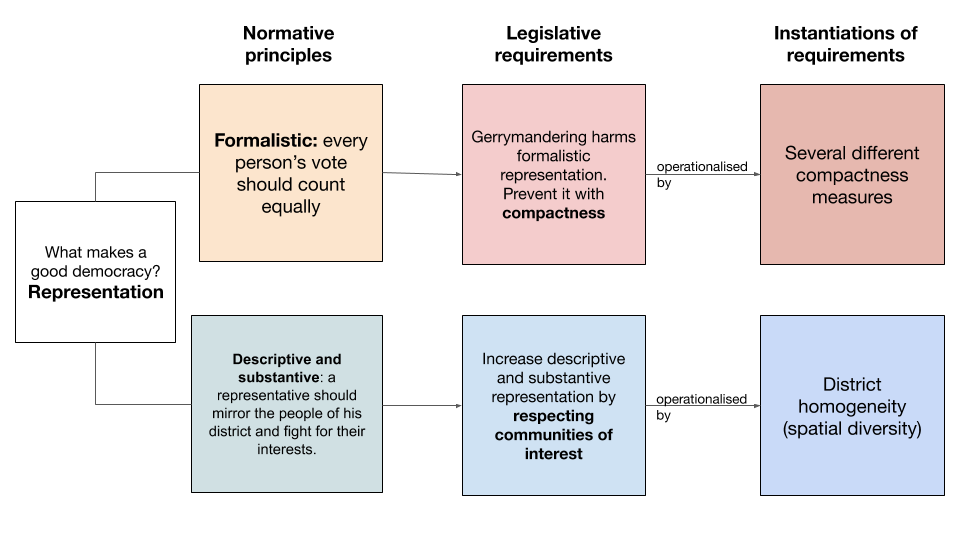
\includegraphics{./img/why_compactness_and_community1.png}
\caption{Why representation matters, and how legislators try to promote
it\label{flowchart}}
\end{figure}

Figure \ref{flowchart} summarises why representation matters, and how
legislators try to promote it. In sum, the normative principle of
representation guides legislators, which try to protect and promote
representation in their constitutions. They do so by mandating that
districts should be ``reasonably compact'' (which protects formalistic
representation) and should respect ``communities of interest'' (which
promotes descriptive and substantive representation). Finally, as the
constitutions do not specify how compactness and communities of interest
should be measured, we must then find a way to operationalise them and
ensure that proposed districting plans comply with them.

However, some have argued that compactness and respecting communities of
interest are fundamentally conflicting goals. After all, communities of
interest do not form neat geometric shapes. For instance---like the
Shenandoah Valley---they may follow a river and be long and serpentine.
In that case, it may be difficult or impossible to draw a compact-enough
plan that does not break up the Valley. \citeauthor{wolf2015} writes
that ``all {[}compactness{]} does is needlessly and unproductively split
communities, cities, and counties''. If so, then mandating compactness
would come at the expense of communities of interest---leaving
redistrictors in an impossible situation.

Is this true? Are more compact districts more likely to split
communities of interest? While many have argued that compactness may
conflict with communities of interest and other desired metrics like
minority vote share and electoral competitiveness (\citep{cain1984},
\cite{karlan1989}), no work that I know of has examined the trade-off
between compactness and communities of interest.

I thus address this open question in this thesis, which investigates the
relationship between two prominent criteria for district design. Using a
simulation approach, I generate many districting plans that represent
the set of plans a non-partisan districting commission pursuing
compactness would possibly generate. I develop a compactness measure of
my own which improves upon existing ones, and see if there is any
correlation between compactness and communities of interest. My results
indicate no trade-off between compactness and homogeneity across all
four compactness measures I examine: plans with more compact districts
do not tend to have lower levels of homogeneity. I further find that my
human compactness measure consistently identifies more homogeneous
districts. Rather than a trade-off, the right choice of compactness
metric can in fact \emph{encourage} keeping communities of interest
together.

\hypertarget{why-compactness-is-important}{%
\subsection{Why compactness is
important}\label{why-compactness-is-important}}

Thirty-seven states require their legislative districts be reasonably
compact, and eighteen states require congressional districts to be
compact as well (Levitt 2019). This is because mandating compactness
prevents gerrymandering, a key way in which incumbents can subvert fair
elections and evade accountability. As \cite{pp1991} put: ``Without the
ability to distend district lines\ldots{} it is not possible to
gerrymander. The diagnostic mark of the gerrymander is the noncompact
district''. This claim is well-supported by the literature:
\cite{apollonio2006} find that ``compactness is a good shield against
the practice of gerrymandering''.

Compactness thus plays a key role in safeguarding formalistic
representation. For this reason, the courts have explicitly used
compactness as a critical desiderata when challenging unrepresentative
plans. \cite{altman1998} writes:

\begin{quote}
In Shaw v. Reno (1993), the Court allowed a challenge to North
Carolina's redistricting plan to proceed on the basis that the
ill-compactness of the districts indicated a racial gerrymander\ldots{}
Bush v. Vera (1996) declares that violations of compactness and other
districting principles are necessary conditions for strict scrutiny to
apply.
\end{quote}

\hypertarget{why-communities-of-interest-are-important}{%
\subsection{Why communities of interest are
important}\label{why-communities-of-interest-are-important}}

Keeping communities of interest together in a district increases
descriptive and substantive representation, which leads to better
democratic outcomes. In this thesis, I use district homogeneity as a
proxy for communities of interest. This is for two reasons: i)
`communities of interest' are ill-defined and difficult to measure; ii)
district homogeneity is regarded as the best proxy for communities of
interest. The evidence suggests that more homogeneous districts have
higher turnout levels, more responsive elections, and representatives
that fight harder for their interests (\cite{steph2012},
\cite{ogrady2018}).

\hypertarget{measuring-communities-of-interest-is-difficult}{%
\subsubsection{Measuring communities of interest is
difficult}\label{measuring-communities-of-interest-is-difficult}}

\citeauthor{altman1998} writes that communities of interest are
important but difficult to pin down:

\begin{quote}
The question of how redistricting in general, and compactness in
particular, affects `communities of interest' is important, but
ill-defined\ldots{} the term is often used when we are unable to more
conventionally classify the `interest' involved. In part because of this
use of `communities of interest' as a catch-all, these communities are
difficult to quantify. The lack of an objective, quantitative, standard
for recognizing such communities makes the subject difficult to examine
through either statistics or simulation.
\end{quote}

We have seen how difficult defining communities of interest can be. In
2010, the California Redistricting Committee made districting maps that
respected ``communities of interest'' through a year-long, drawn-out
process, which involved recruiting unbiased candidates to form the
committee, holding dozens of public input hearings, reading through
comments and suggestions from over 20,000 individuals and groups, and
conducting hundreds of field interviews. It relied on the ``active
participation'' of citizens across California to weigh in on an ``open
conversation'' in which ``{[}the commission{]} deliberated over the best
approach to minimize the splitting of cities, counties, neighbourhoods,
and local communities of interest''. While this approach did succeed in
identifying communities of interest, the Herculean effort involved makes
it unlikely to be replicated in other states. More recently, the MGGG
Redistricting Lab built a tool inviting members of the public to tag and
identify communities of interest---because ``communities of interest are
notoriously hard to locate'' \citep{mggg2020}.

\hypertarget{using-district-homogeneity-as-a-proxy}{%
\subsubsection{Using district homogeneity as a
proxy}\label{using-district-homogeneity-as-a-proxy}}

As communities of interest are hard to define and hard to measure, I use
district homogeneity---how similar people in a district are, measured on
key demographic indicators---as a proxy instead. District homogeneity
tracks communities of interest quite closely. The idea is simple: people
in the same ``communities of interest'' are often more alike than not:
for instance, they may often be of the same age group, race, or
religion. In fact, communities of interest are often viewed through
exactly that lens. The Constitution of Colorado defines communities of
interest as ``ethnic, cultural, economic, trade area, geographic, and
demographic factors'', and Massachussets defines them based on ``trade
areas, geographic location, communication and transportation
networks\ldots{} social, cultural and economic interests, or occupations
and lifestyles'' \citep{brennan}.

Unlike communities of interest, moreover, there is broad agreement on
what homogeneity constitutes. I use American Community Survey (ACS)
data---which contains all sorts of demographic data like educational
attainment, income, employment, housing, age, race, and so on---at a
geographic (Census Tract) level. These are regarded as the ``best
available proxies for how closely\ldots{} districts correspond to
\emph{geographic communities of interest}'' \citet[p.~283]{steph2012}.

I operationalise district homogeneity using a particular instantiation
called \emph{spatial diversity} developed by \cite{steph2012}. It
measures the variance in each Census Tract along ACS factors such as
race, ethnicity, age, income, education, and so on. The higher the
spatial diversity score, the less homogeneous the district.

\hypertarget{district-homogeneity-is-associated-with-better-democratic-outcomes}{%
\subsubsection{District homogeneity is associated with better democratic
outcomes}\label{district-homogeneity-is-associated-with-better-democratic-outcomes}}

\begin{figure}
\centering
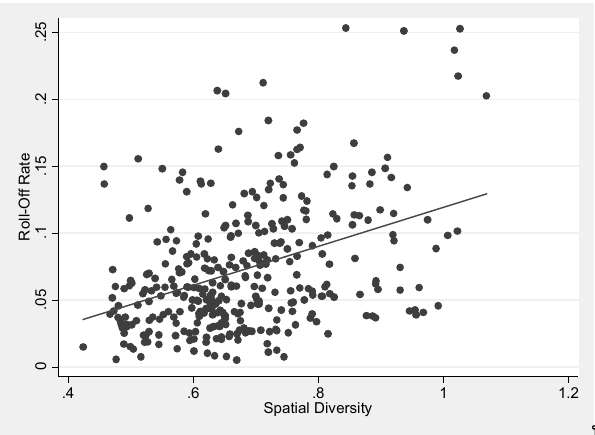
\includegraphics{img/sd_rolloff.png}
\caption{Increased spatial diversity (lower homogeneity) is associated
with an increase roll-off rate \label{sd_rolloff}}
\end{figure}

In accordance with the evidence presented so far, Stephanopoulos finds
that district homogeneity and statewide homogeneity are both strong
predictors of democratic outcomes. Figure \ref{sd_rolloff} shows the
relationship between spatial diversity and roll-off rate, which is
defined as the difference between the proportion of voters who cast a
ballot for a presidential race and the proportion who cast a ballot for
a lower-ticket (e.g.~Congressional) race. Roll-off rates are important
indicators of democratic participation, because they zero in on the
confusion, lack of knowledge, or apathy that prevents voters from
casting their vote in the Congressional race despite having cast a
top-ticket vote. Stephanopoulos argues that increasing spatial diversity
increases the roll-off rate, which makes sense given what we know so
far: homogeneous districts are easier to represent and representatives
can better act in their constituents' interests.

\begin{figure}
\centering
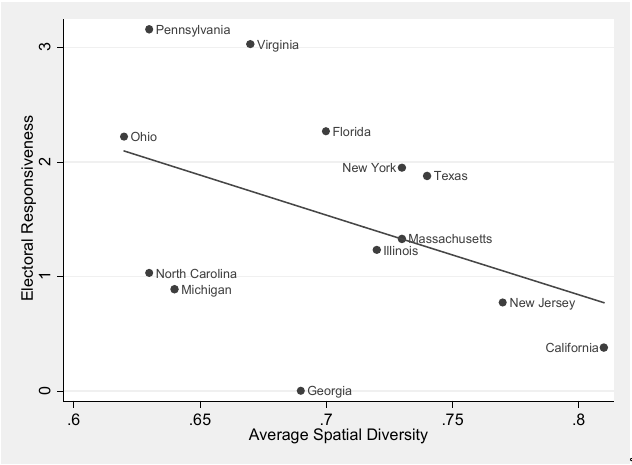
\includegraphics{./img/average_spatial-diversity.png}
\caption{Relationship between spatial diversity and electoral
responsiveness\label{sd_responsiveness}}
\end{figure}

Stephanopulos finds that homogeneous districts also tend to be the ones
whose elections are most responsive to changes in public opinion. Figure
\ref{sd_responsiveness} plots the relationship Stephanopoulos found
between spatial diversity and electoral responsiveness. Electoral
responsiveness refers to the rate at which a party gains or loses seats
given changes in its statewide vote share. For instance, if Democrats
would win ten percent more seats if they received five percent more of
the vote, then a plan would have a responsiveness of two. The higher a
plan's responsiveness, the better it is thought to be. Stephanopoulos
finds that more homogeneous districts are more responsive, and writes
that ``advocates of responsive elections\ldots{} may push without
hesitation for spatially homogeneous districts to be drawn''.

In sum, district homogeneity is associated with a variety of positive
democratic outcomes.

\hypertarget{a-conflict-between-compactness-and-communities-of-interest}{%
\subsection{A conflict between compactness and communities of
interest?}\label{a-conflict-between-compactness-and-communities-of-interest}}

In the previous section, I have established that both compactness and
communities of interest are greatly cherished by legislators. However,
some have argued that compactness and respecting communities of interest
are fundamentally conflicting goals. In order to form districts that are
compact enough, a districting commission may have to break apart
communities of interest, or agglomerate two communities with nothing in
common except that they fit neatly into a neat geometric shape.

Some communities of interest like the Shenandoah Valley may follow a
river and be long and serpentine. In that case, it may be difficult or
impossible to draw a compact-enough plan that does not break up the
Valley. \citeauthor{wolf2015} writes that ``all {[}compactness{]} does
is needlessly and unproductively split communities, cities, and
counties''. If so, then mandating compactness would come at the expense
of communities of interest---leaving redistrictors in an impossible
situation.

Previous work has found trade-offs between compactness and other
democratic outcomes. \cite{ddj2019comp} show that mandating
competitiveness has effects on the partisan lean of the ensuing
districting plans. And \cite{s2020} finds that compactness and partisan
symmetry (competitiveness) are somewhat incompatible, suggesting that
mandating compactness may have unwanted effects on desired electoral
outcomes. It is therefore plausible, as many have suggested, that there
is also a trade-off between compactness and communities of interest.

\hypertarget{key-research-questions}{%
\section{Key research questions}\label{key-research-questions}}

Can we have plans that are both very compact and respect communities of
interest? Is there a trade-off between community and compactness?
Additionally, while legislators have mandated that districting plans be
``reasonably compact'', they have not specified how compactness should
be measured. There are dozens of compactness measures that have been
proposed in the literature: if there is indeed a trade-off, might some
of them be able to better accommodate both compactness and community?

Along these lines of thought, I pose the following research questions:

\hypertarget{is-there-a-trade-off-between-compactness-and-communities-of-interest}{%
\subsection{Is there a trade-off between compactness and communities of
interest?}\label{is-there-a-trade-off-between-compactness-and-communities-of-interest}}

Many have claimed that mandating compactness may lead to districts that
split communities of interest. But while \emph{some} very compact
districts may split communities, there may also be very compact
districts that do not. The key question is this. Within the set of plans
that an unbiased redistrictor could draw, do more compact plans tend to
be more or less homogeneous? Is there a tradeoff between compactness and
community?

\hypertarget{do-some-compactness-metrics-better-encompass-communities-of-interest-than-others}{%
\subsection{Do some compactness metrics better encompass communities of
interest than
others?}\label{do-some-compactness-metrics-better-encompass-communities-of-interest-than-others}}

While almost all states mandate that districts are drawn in a
``reasonably compact'' fashion, they do not specify \emph{how}
compactness should be measured. A natural question is to ask which
compactness measures we should choose from the dozens proposed in the
literature.

While there may be theoretical and methodological reasons to favour one
compactness measure over another, there is also a normative
consideration. If the plans favoured under one compactness measure are
consistently more homogeneous than the others, then this might give us a
normative basis for choosing amongst the different compactness measures.

\hypertarget{methodology}{%
\section{Methodology}\label{methodology}}

To answer my research questions, I adopt the following research
procedure:

\begin{enumerate}
\def\labelenumi{\arabic{enumi}.}
\tightlist
\item
  Generate a large and representative subset of plausible districting
  plans
\item
  Evaluate compactness and spatial diversity scores on that subset of
  plans
\item
  Analyse the overall relationship between compactness and communities
  of interest (operationalised by spatial diversity)
\end{enumerate}

This three-step procedure is used by many previous works, including
\cite{cr2013}, \cite{ddj2019comp}, and \cite{s2020}. While the specifics
differ, they all follow the same general procedure. I now explain why
this procedure (analyzing hypothetical districting plans) has advantages
over analyzing enacted or proposed districting plans.

\hypertarget{why-a-simulation-approach-is-necessary}{%
\subsection{Why a simulation approach is
necessary}\label{why-a-simulation-approach-is-necessary}}

I use a simulation approach to generate tens of thousands of plausible
districting plans. One might ask: What is the point of using a
simulation approach? Why not just use historical districting plans that
actually existed in real life? There are two reasons. Firstly, there
have not been very many historical districting plans. There may be at
most twenty districting plans over the history of a state, but they
range from the 1800s to the 2000s. It would be difficult to get
geospatial data on these historical plans, and impossible to get any
demographic data on district homogeneity/communities of interest.

But the biggest problem in trying to draw a link between districting
plans and any outcome of interest is that of endogeneity. Suppose we
believe that less compact plans lead to less political participation:

\[Compactness \rightarrow Participation\]

To identify whether this relationship is true, we could look at several
enacted districting plans and measure their compactness and political
participation. Then we would be able to run an OLS regression and
retrieve the coefficients. But these coefficients would not have a
causal interpretation. We know that compactness is a result of
districting procedures that are political in nature. Political
participation affects who wins the state, and the winning party then has
outsize influence on the next districting plan. The districting plans
affect the outcome of the election, which in turn affects future
districting plans. This makes it difficult to find the marginal effect
of an increase in compactness on participation.

Even finding natural experiments may not be enough to remove the
endogeneity. The Supreme Court has often struck down proposed
districting plans and forced parties to propose a new one. We can think
of this as an exogenous shock and calculate compactness and political
participation in both plans. But even this has knock-on effects. When
the Supreme Court strikes down a plan, it's safe to say that there will
be significantly increased media coverage on the proceedings---which
will surely affect interest and participation in the subsequent
elections.

It would be useful to vary compactness unilaterally while knowing that
that variation was not due to a previous change in political
participation. But this is precisely what simulation approaches allow us
to do. If we could simulate plans that represent the set of plans that a
non-partisan committee pursuing compactness might generate, then we
would solve the problems of small sample size, lack of data, and
endogeneity in one fell swoop.

A simulation approach is therefore advantageous due to the limitations
of our data. But the simulation procedure introduces several new
considerations. We need to choose two things in the procedure: a method
to generate districting plans, and a compactness metric to score these
districting plans. This choice highly consequential: different
generating functions and the choice of compactness metric can give very
different results. I now explain how I chose both of these.

\hypertarget{choosing-which-compactness-measures-to-evaluate}{%
\subsection{Choosing which compactness measures to
evaluate}\label{choosing-which-compactness-measures-to-evaluate}}

To empirically evaluate a trade-off between compactness and homogeneity,
we must first figure out how to measure compactness. I give a brief
overview of the different types of measures and explain the pros and
cons of each. I present a compactness measure that I develop and finally
explain my decision to analyse four different compactness measures to
increase the robustness of my results.\footnote{I use the phrases
  ``compactness metric'' and ``compactness measure'' interchangeably.}

Over a hundred compactness measures have been proposed in the
literature. Here, I focus on two main families: \emph{geometric}
compactness metrics and \emph{point-wise distance} metrics.

\hypertarget{geometric-compactness-metrics}{%
\subsubsection{Geometric compactness
metrics}\label{geometric-compactness-metrics}}

Geometric compactness metrics are by far the largest class of
compactness measures. They look at some geometric properties of proposed
districts. These properties are most often shapes, area or
perimeter---although more esoteric measures do exist. Here, I explain
the three most popular compactness measures, although other popular
compactness measures e.g.~Schwartzberg are qualitatively similar.

\hypertarget{polsby-popper}{%
\paragraph{Polsby-Popper}\label{polsby-popper}}

The Polsby-Popper measure is by far the most popular measure used in the
literature. It is the ratio of the area of the district to the area of a
circle whose circumference is equal to the perimeter of the district
\citep{pp1991}. A perfect circle has a Polsby-Popper score of 1.

\[4\pi \times \frac{A}{P^2}\]

\begin{figure}
\centering
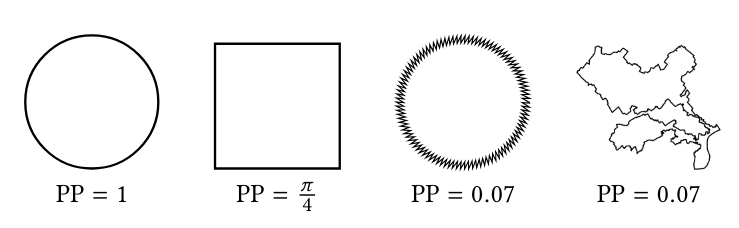
\includegraphics{img/pp_example.png}
\caption{Polsby-Popper scores of four example districts: a perfect
circle, a square, a circle with a ragged boundary, an an example
district from a Pennsylvania plan. Taken from \cite{s2020}.}
\end{figure}

\hypertarget{reock}{%
\paragraph{Reock}\label{reock}}

The Reock score is the ratio of the district's area to the area of the
minimum bounding circle that encloses the district's geometry
\citep{reock1961}.

\[\frac{Area}{AreaOfMinimumBoundingCircle}\]

\begin{figure}
\centering
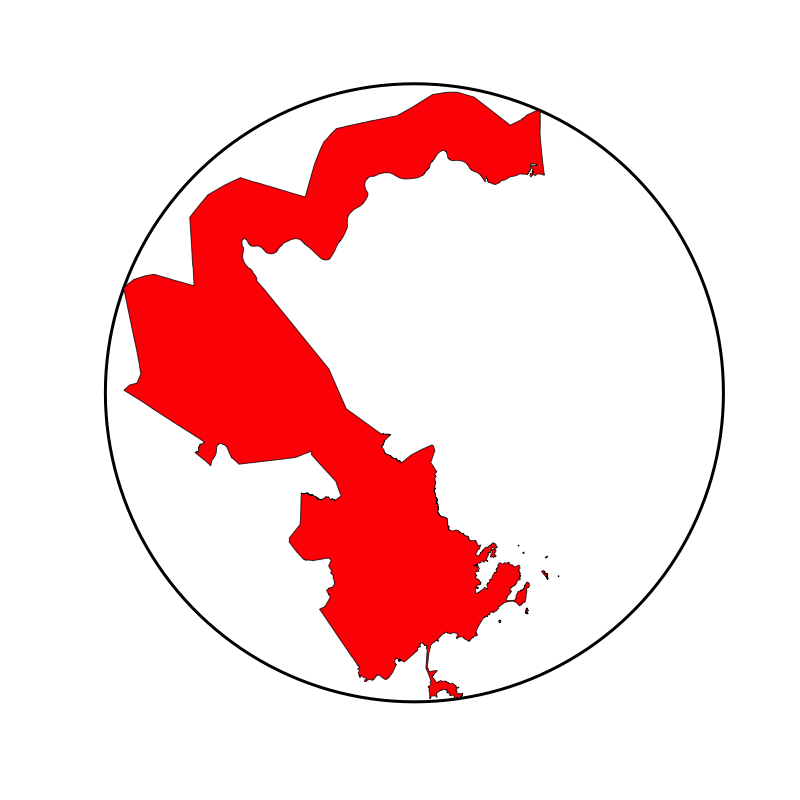
\includegraphics{img/reock.png}
\caption{A visualisation of the Reock metric.}
\end{figure}

\hypertarget{convex-hull}{%
\paragraph{Convex Hull}\label{convex-hull}}

The Convex Hull metric is a ratio of the area of the district to the
area of the minimum convex polygon that can enclose the district's
geometry. A circle, square, or any other convex polygon has the maximum
Convex Hull score of 1.

\[\frac{Area}{AreaOfMinimumConvexPolygon}\]

\begin{figure}
\centering
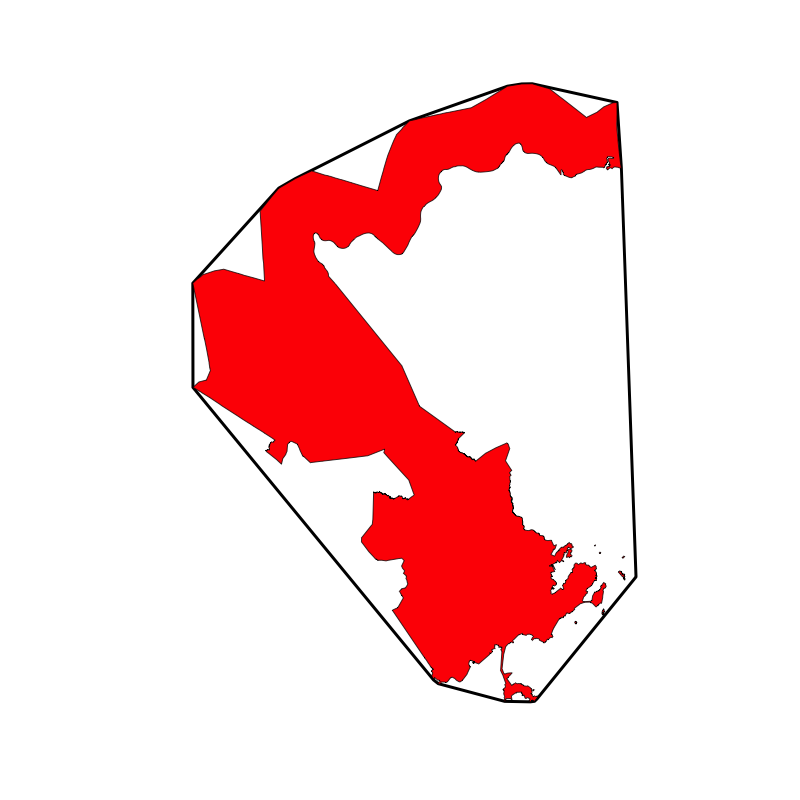
\includegraphics{img/ch.png}
\caption{A visualisation of the Convex Hull metric.}
\end{figure}

\hypertarget{point-wise-distance-compactness-measures}{%
\subsubsection{Point-wise distance compactness
measures}\label{point-wise-distance-compactness-measures}}

Another large family of compactness measures are \emph{non-geometric
measures}, which do not take into account the geometric properties
(e.g.~area, perimeter) of the district explicitly. Many such
non-geometric measures have been proposed. For instance, \cite{dc2016}
bring in a discipline of mathematics---graph theory---to formulate a new
metric of compactness. And \cite{kingwp} use a machine learning model to
try and ape human intuition---quantifying the intuitive metric of ``I
know it when I see it''.\footnote{This penalises districting plans that
  have a large difference between districts e.g.~one very good district
  and one very bad one.}

But one particular class of metrics I term \emph{point-wise distance}
compactness stands out for its ease of understanding (critical if it is
to be persuasive to Supreme Court judges), theoretical attractiveness,
and academic consensus. Roughly speaking, this class of compactness
metrics tries to measure the distance between voters in a district, and
assigns higher scores the lower that distance is.

This class of metrics enjoys strong theoretical grounding. Paramount to
the idea of single-member districts is that there is some value in
voters who live in the same area being put into the same district.
\cite{er2019} write:

\begin{quote}
``Voters in the same area are likely to share political interests;
voters in the same area are better able to communicate and coordinate
with one another; politicians can better maintain connections with
voters in the same area; voters in the same area are especially likely
to belong to the same social communities --- all suggest the importance
of voters being located in districts with their geographic peers.''
\end{quote}

A wealth of empirical evidence supports the above statement.
\cite{arzheimer2012} find that constituents support less strongly
candidates that live far from them, even controlling for strong
predictors of vote choice like party feeling and socio-economic
distance. Similarly, \cite{dyck2005} find that voters living further
away from a voting site are less likely to turn out to vote. In part,
voters strongly support proximate candidates because they think that
these candidates better represent their interests. If voters prefer a
representative who lives close to them, then we can satisfy the most
voters by drawing districts where everyone lives close to everyone
else---only then can that district have a representative who lives close
to everybody.

In contrast, districts that put people with unrelated, faraway others
carve voters out of their natural communities and are thus to be
avoided. We care about whether co-districtors live in the same area and
belong to the same communities of interest, not just the compactness of
their electoral district. And point-wise distance metrics deliver
exactly that.

Therefore, point-wise distance metrics are more intuitive to laymen and
possess a normative bent that more abstract mathematical compactness
measures lack. It has therefore been an active area of development in
the literature. \cite{cm2010} present a measure of ``bizarreness'',
which is the ``expected relative difficulty in traveling between two
points within the district''. And \cite{fh2011} measures ``the distance
between voters within the same district relative to the minimum distance
achievable''.

\hypertarget{flaws-with-existing-compactness-metrics}{%
\subsubsection{Flaws with existing compactness
metrics}\label{flaws-with-existing-compactness-metrics}}

In this section, I show existing compactness metrics are useful but
somewhat inadequate. Geometric compactness measures have several
well-known problems, and while point-wise distance metrics fix many of
these problems, they have issues of their own. I thus develop a new
compactness metric which improves upon existing point-wise distance
metrics.

All three geometric compactness measures are well-cited in the
literature and enjoy widespread use. They have been cited in U.S.
Supreme Court cases, \emph{amici} briefs, and redistricting commissions
\citep{moncrief2011}. Despite their widespread use, however, the
problems with compactness measures are many, and well-covered in the
literature. As an example, the most popular compactness measure in the
literature---Polsby-Popper---is sensitive to small perturbations in data
resolution (the coastline problem).\footnote{The Polsby-Popper metric
  measures the ratio of the area of the district to the area of a circle
  whose circumference is equal to the perimeter of the district. But
  depending on the resolution of the map, the perimeter can be
  effectively infinite. \citeauthor{bswp} find that the choice of
  resolution has ``a substantial impact on compactness scores, with the
  Polsby-Popper score especially affected.''} The same is true for other
geometric compactness measures: no single metric is perfect.

Because all three of these compactness measures are purely geometric,
they are all vulnerable to geographic perturbations. Indeed, \cite{bswp}
show that minimal changes in the geometric features of states are enough
for the four most popular compactness measures (Polsby-Popper, Convex
Hull, Reock, Schwartzberg) to give very different conclusions on
nominally identical data. These changes do not have to be made on
purpose: small changes in the way the data is collected or processed can
suffice to affect the conclusions we draw.

And despite the relative merits of point-wise distance metrics, there
are two areas of improvement---one theoretical, the other empirical.
Firstly, all point-wise distance metrics suggested in the literature use
Euclidean distances. But many have rightly suggested that we should
consider travel times/driving durations instead. For instance, while
\cite{fh2011} used Euclidean distance in their metric, they point out
its shortcomings:

\begin{quote}
Suppose there is a city on a hill. On the West side is {[}a{]} mild,
long incline toward the rest of the city, which is in a plane. On the
East side is a steep cliff, either impassable or with just a narrow,
winding road that very few people use. While the next residential center
to the East is much closer to the hilltop on a horizontal plane, it is
much further on all sorts of distances that we think might matter:
transportation time, intensity of social interactions, sets of shared
local public goods and common interests, etc. Thus, for all practical
purposes, one probably wants to include the hilltop in a Western
district rather than an Eastern one. More general notions of distance
can handle this.
\end{quote}

Here we see the key problem with using Euclidean distances in point-wise
distance metrics. The ``impassable'' region on the East would have a
short Euclidean distance, and any districting plan that put the hilltop
with the Eastern district would be unfairly penalised by these
point-wise distance metrics. Evidently, using driving durations instead
would give us more accurate scores. Using driving durations, the
impassable region would have a long driving duration, accurately
reflecting the political geography. In this and many other cases like it
(e.g.~large bodies of water), driving durations better reflect a state's
unique political geographies.

After acknowledging the shortcomings of Euclidean distance,
\citeauthor{fh2011} specifically suggest using driving durations to
improve their metric: ``one can extend much of {[}our analysis{]} by
using driving distance or what legal scholars refer to as `communities
of interest'\,''.

There are thus strong theoretical grounds for using driving durations in
point-wise distance metrics. Why then have scholars not adopted it,
seeing as they agree on its superiority? This brings me to my empirical
criticism: the point-wise distance metrics scholars have proposed are
either far too computationally complex to compute at scale, or have
restrictions that make using travel times difficult, if not impossible.
For instance, the metric that \citet{fh2011} propose requires solving an
\emph{NP-complete} problem. A term used in computer science, an
NP-complete problem scales exponentially with the size of the input.
This makes it prohibitively expensive on larger states. And while they
have an approximation that runs much quicker, they provide no bounds on
the correctness of this approximation.

Similarly, \citeauthor{olson2010} has a metric that minimises the
average distance from each voter to the center of their district. He
says of travel times ``that it might be the right kind of thing to
measure, but it would take too long\ldots{} The large amount of map data
and extra computer time to calculate all those travel times would slow
the process down horribly. It would then require a room filling
supercomputer to get an answer in a reasonable amount of time.''
\citep{olson2010}. And finally, \citeauthor{cm2010}'s measure cannot
feasibly be improved with driving durations due to the difficulty of
finding point-to-point travel distances without passing through another
district. This is because most routing engines allow you only to specify
a route between two (or more) points. They do not further allow you to
specify regions through which the route cannot pass.

\hypertarget{building-a-new-compactness-metric-human-compactness}{%
\subsubsection{Building a new compactness metric: Human
compactness}\label{building-a-new-compactness-metric-human-compactness}}

Given the difficulties of adapting existing point-based distance metrics
to use driving durations, I develop a new measure called \emph{human
compactness}. This metric incorporates driving durations at the very
outset, and builds in optimisations to run quickly. The human
compactness metric measures the ratio of driving durations between one's
nearest neighbours and one's fellow districtors. This ratio ranges from
0 to 1. The higher this ratio is, the more compact the district.
Intuitively, it encourages drawing districts that put one's next-door
neighbours together in the same district.

The human compactness metric works at three levels: at the voter-level,
the district-level, and the overall plan-level. At the voter level,
human compactness of a voter is the ratio of: the sum of driving
durations to one's K nearest neighbours, to the sum of driving durations
to one's co-districtors, where K is the number of voters in that voter's
district.

A simple example will be illuminating. The following figures give a
simple demonstration of how the human compactness metric is calculated
both on the voter- and district- level. The example works for both
Euclidean distances and driving durations: only a simple swap is
required.

\begin{figure}
\centering
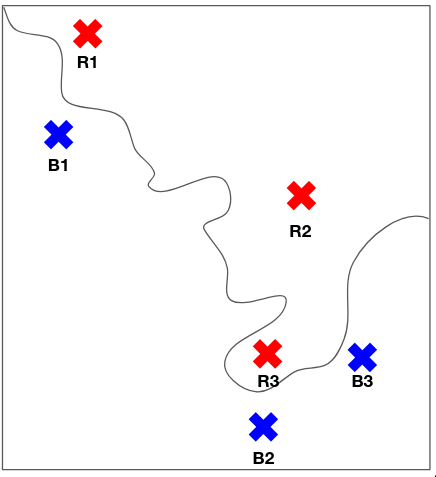
\includegraphics{img/human_compactness_1.png}
\caption{A simplified state assignment with two districts and six voters
\label{hc_demo}}
\end{figure}

Figure \ref{hc_demo} shows a highly simplified state assignment, with
two districts, Red and Blue, and three voters in each district. We label
each point from top-left to bottom-right. Note here that Red and Blue
are not partisan affliations: R1, R2 and R3 are red voters simply
because they happen to fall in the Red district.

We will first calculate the individual human compactness score for each
voter in the Red district. Figure \ref{hc_r1} illustrates this for the
top-left voter, R1. First, we find the sum of distances between R1 and
his fellow co-districtors R2 and R3. This sum, \(5 + 6\), forms the
denominator of the human compactness score.

\begin{figure}
\centering
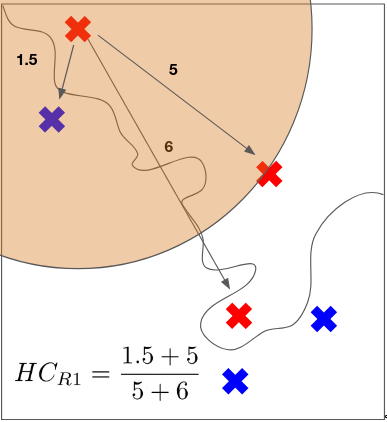
\includegraphics{img/human_compactness_2a.png}
\caption{Human compactness measure for voter R1 \label{hc_r1}}
\end{figure}

Next, we find the sum of driving durations between R1 and his nearest
neighbours. Because there are two other voters in his district, we will
find his two nearest neighbours. To find the two nearest neighbours,
here I have drawn a circle centered upon R1, and expanded the circle on
all sides until it touches two other voters.\footnote{The method of
  drawing an ever-expanding circle to get one's K-nearest neighbours
  only works for Euclidean distances. In reality, the ``circle of
  K-nearest neighbours'' will not be a circle, but rather be what is
  called an \emph{isochrone}: a line drawn on a map that connects points
  that have the same travel duration. The shape of the isochrone will
  vary with geographic features like cliffs or man-made features like
  highways. My implementation of the human compactness algorithm
  precomputes all the K-nearest neighbours for every single point,
  negating the need to calculate isochrones.}. We can see that R1's
nearest neighbours are the points B1 and R2, with a distance of 1.5 and
5 respectively. The human compactness score of R1 is thus
\[HC_{R1} = \frac{d_{B1}+d_{R2}}{d_{R2} +
d_{R3}} = \frac{1.5 + 5}{5+6} = 0.59\]

\begin{figure}
\centering
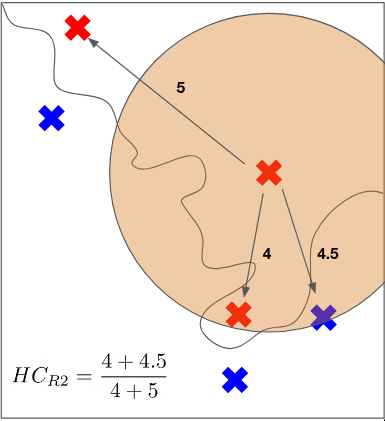
\includegraphics{img/human_compactness_2b.png}
\caption{Human compactness measure for voter R2 \label{hc_r2}}
\end{figure}

This is how we calculate an individual human compactness score. We
repeat the same procedure with R2 and R3, and obtain
\(HC_{R2} = \frac{4 + 4.5}{5+4}=0.94\) and
\(HC_{R3} = \frac{2 + 2.5}{4+6} = 0.45\). The compactness score for
point R3 is particularly low. We can see why this is the case in Figure
\ref{hc_r3}. Because point R3 is so close to B2 and B3, it really should
be put in the same district with them---R3 likely lives in the same
neighbourhood and/or community as B2 and B3. This is why the human
compactness metric gives it a very low score.

\begin{figure}
\centering
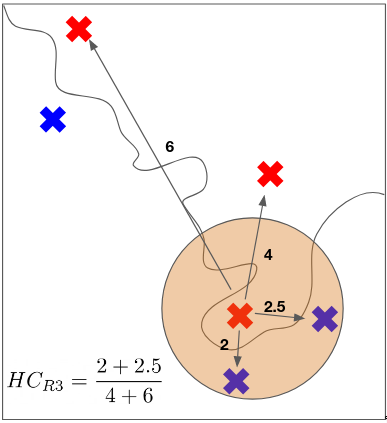
\includegraphics{img/human_compactness_2c.png}
\caption{Human compactness measure for voter R3 \label{hc_r3}}
\end{figure}

The \emph{district's} human compactness measure, \(HC_R\), simply takes
the ratio of all the sum of durations, as follows:\footnote{Another
  reasonable approach might be take the arithmetic mean of all
  individual human compactness scores. In that case the district-level
  human compactness score would be \(0.59 + 0.94 + 0.45 / 3 = 0.66\),
  basically identical to the value we obtained.}

\[HC_R = \frac{(1.5+5) + (4 + 4.5) + (2.5 + 2)}{(5+6) + (5+4) + (4+6)} =
0.65\]

Finally, we obtain the districting plan's \emph{plan-level} compactness
score by taking the simple arithmetic mean of all district-level
compactness scores. Other aggregation functions are plausible: for
instance, taking the median, or the root-mean-squared value. In the
Results section, I run robustness checks with the root-mean-squared
aggregation function and find qualitatively similar results.

\begin{figure}
\centering
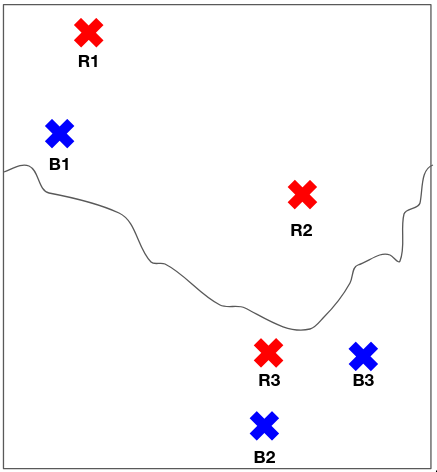
\includegraphics{img/human_compactness_3.png}
\caption{An alternative, more humanly compact proposed districting plan
\label{hc_better}}
\end{figure}

We have seen how to calculate the human compactness score for a proposed
districting plan. Now we demonstrate the conditions under which human
compactness score will assign better scores.

Figure \ref{hc_better} shows a proposed alternative districting plan.
Only the boundary has changed---the points have not. We can see
intuitively that this plan is more compact. Rather than being ``carved
out'' of his natural community in a snakelike fashion, R3 is now put in
a reasonably-shaped district with B2 and B3. We can calculate the
spatial diversity of this new district by imputing reasonable distance
values for R1--B1 and R2--B1. We thus get

\[HC_{R*} = \frac{(1.5 + 5) + (1.5+4.5) + (4 + 4.5)}{(1.5+5) + (1.5+4.5) + (5+4.5)} = 0.95\]

As we can see, the new district (and by extension districting plan) is
given a much higher score under the human compactness metric, which
largely accords with our intuitions. The human compactness measure
enjoys two significant advantages over existing approaches. First, the
human compactness metric improves upon the algorithmic complexity of
\citeauthor{fh2011}'s algorithm from an NP-hard problem to one with a
\(O(n^2)\) polynomial runtime. This is an exponential decrease in
algorithmic complexity. I also use programming techniques like
precomputation and memoisation to decrease the time taken to compute the
metric greatly. My implementation is competitive with geometry-based
compactness measures like Reock: on my machine, both metrics took
roughly the same amount of time (\textasciitilde{}0.20s per step). This
greatly increases the capability of political science researchers to
conduct ensemble analysis without requiring ``room-filling
supercomputers''. Further details on these algorithmic optimisations can
be found in Technical Appendix B.

Because of these algorithmic improvements and the way I have designed
the metric, I am able to use driving durations rather than Euclidean
(as-the-crow-flies) distances between voters. This is a large
improvement with strong theoretical and empirical support. Many previous
scholars have suggested exactly this, giving it strong theoretical
support. It keeps the metric robust to quirks in political geography
like mountains and lakes, and better represents the notion of natural
communities.

\begin{figure}
\centering
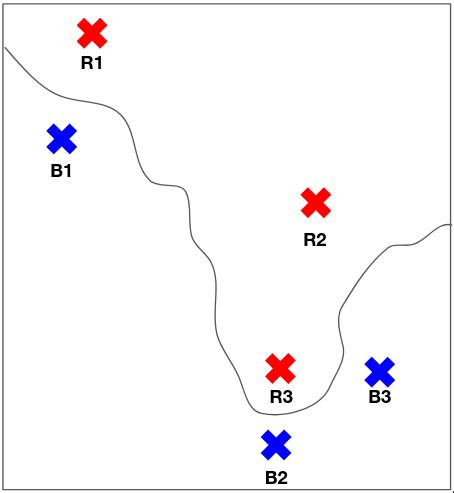
\includegraphics{./img/hc_impassable.jpg}
\caption{With an impassible cliff face, Euclidean distance gives the
wrong answer \label{hc_impassible}}
\end{figure}

Figure \ref{hc_impassible} shows how driving durations is able to get
the right answer despite quirks in political geography. It represents
the situation that \cite{fh2011} point out: the voters in red live atop
a cliff, and the valley below (inhabited by the voters in blue) is
impassible. In this case, it would be better to put the voters in red
together, as they are ``closer'' together on all sorts of metrics that
would matter: shared communities, public services, and so on. A
compactness measure that used Euclidean distances would not be able to
accommodate this.

Empirically, too, the use of driving durations seems strictly superior
in many cases involving human-scale distances. Working with Eubank and
Rodden, I update their gerrymandering-detection metric to use driving
durations instead \citep{er2019}. We find a consistently different
picture of the social context of American suburban voters, raising the
possibility of false positives under the Euclidean distance measure
\citep*{elrwp}.

\hypertarget{choosing-which-compactness-metrics-to-evaluate}{%
\subsubsection{Choosing which compactness metrics to
evaluate}\label{choosing-which-compactness-metrics-to-evaluate}}

As each compactness measure has its advantages and disadvantages, we
should include the broadest subset of measures possible in my analyses.
This will also maximise the generalisability of my results: in order to
claim that there is or isn't a tradeoff between compactness and
homogeneity, we should make sure that the relationship holds for as many
compactness measures as possible. At the same time, though, the
inclusion of each additional compactness measure incurs time, effort and
computational costs. Given finite time and resources, there is thus a
trade-off between the number of compactness measures and the number of
states/districting plans I can analyse. I therefore made a judgement
call to include the most-used and most representative compactness
measures.

Without question, we must include at least one of the geometric
compactness measures. This is because these geometric compactness
measures are by far the most widely used, both inside academic political
science and out. As mentioned, they have been cited in U.S. Supreme
Court cases, \emph{amici} briefs, and redistricting commissions
\citep{moncrief2011}. I therefore include the three most popular
geometric compactness measures (Polsby-Popper, Convex Hull, and Reock).

It is also important to include a non-geometric compactness measure as
the geometric compactness measures are all sensitive to small changes in
the way the geospatial data are collected and processed.

I use my human compactness measure as a representative of non-geometric
compactness measures, for two reasons. Firstly, many of the compactness
measures have a formal mathematical definition but have no code
available online. It would have taken too much time for me to
re-implement the compactness measure and calculate it for 100,000
districting plans. Secondly, human compactness is the only measure that
incorporates travel durations, which has strong theoretical/normative
backing and some tentative empirical support. Nonetheless, I would have
liked to include another non-geometric compactness measure.

Given these considerations, I settle on using four different compactness
measures: Polsby-Popper, Reock, Convex Hull, and Human Compactness.

\hypertarget{choosing-an-algorithm-to-generate-districting-plans}{%
\subsection{Choosing an algorithm to generate districting
plans}\label{choosing-an-algorithm-to-generate-districting-plans}}

In order to find out whether compactness measures track spatial
diversity, we have to generate many districting plans that span the set
of plans a nonpartisan districtor would draw. We would then measure the
correlation between compactness and spatial diversity. This requires
using a computer to draw a large number of plans, and I use a simulation
approach to do so.

How should we draw the representative plans? Many approaches have been
suggested in the computational districting literature (\cite{ccd2000},
\cite{cr2013}, \cite{fifieldwp}, \cite{ddj2019recom}). I have chosen a
simulation approach known as Markov Chain Monte Carlo (MCMC). This
approach generates many plausible districting plans, then accepts and
rejects them based on a ``score function''. I deliberately chose an
approach with a very permissive score function (a ``neutral ensemble''
approach). Unlike other approaches, my approach does not impose any
additional requirements like county boundaries, proportionality, or
minority deviation. The only requirements on plans are that they fulfill
minimal population deviation and compactness requirements. This is to
ensure that the algorithm generates the subset of plans most
representative of what a nonpartisan districting commission would.
Additionally, my chosen approach is regarded as the state-of-the-art in
the computational redistricting literature \citep{ddj2019recom}.

The details of how I chose the algorithm are in Technical Appendix A. I
start with a literature review of seminal work in computational
districting and evaluate three different state-of-the-art MCMC
approaches before choosing my preferred one (neutral ensemble +
\texttt{ReCom} proposal).

\hypertarget{research-procedure}{%
\section{Research procedure}\label{research-procedure}}

Now that we have chosen both the compactness metric and the simulation
procedure, we can refine the previous three-step procedure into
something more specific:

\begin{enumerate}
\def\labelenumi{\arabic{enumi}.}
\tightlist
\item
  Use the MCMC simulation algorithm to generate 10,000 districting plans
  for every state
\item
  Calculate spatial diversity and four compactness scores
  (Polsby-Popper, Reock, Convex Hull, and Human Compactness) for each
  districting plan
\item
  Perform data analysis (OLS regressions, difference-in-means test) and
  analyse the results
\end{enumerate}

I now describe each step in detail.

\hypertarget{generating-100000-districting-plans-with-the-mcmc-algorithm}{%
\subsection{Generating 100,000 districting plans with the MCMC
algorithm}\label{generating-100000-districting-plans-with-the-mcmc-algorithm}}

I download Census Tract data from the \href{census.gov}{United States
Census Bureau} website. I use Census Tracts rather than Census Blocks
because Census Tracts are the smallest (highest-resolution) units that
have spatial diversity data.

I use the open-source software library GerryChain to generate the
ensembles. Replication code and data are included in my GitHub
repository. I obtain the ReCom Markov chain procedure from one of the
co-authors (Daryl Deford) of the \cite{ddj2019recom} paper. I then fed
the Census Tract data into the GerryChain library. Using the Recom
Markov chain procedure, I generated 10,000 districting plans for 10
states (Connecticut, Georgia, Idaho, Louisiana, Maine, Maryland, New
Hampshire, Rhode Island, Utah, and Wisconsin) for a total of 100,000
plans.

\begin{figure}
\centering
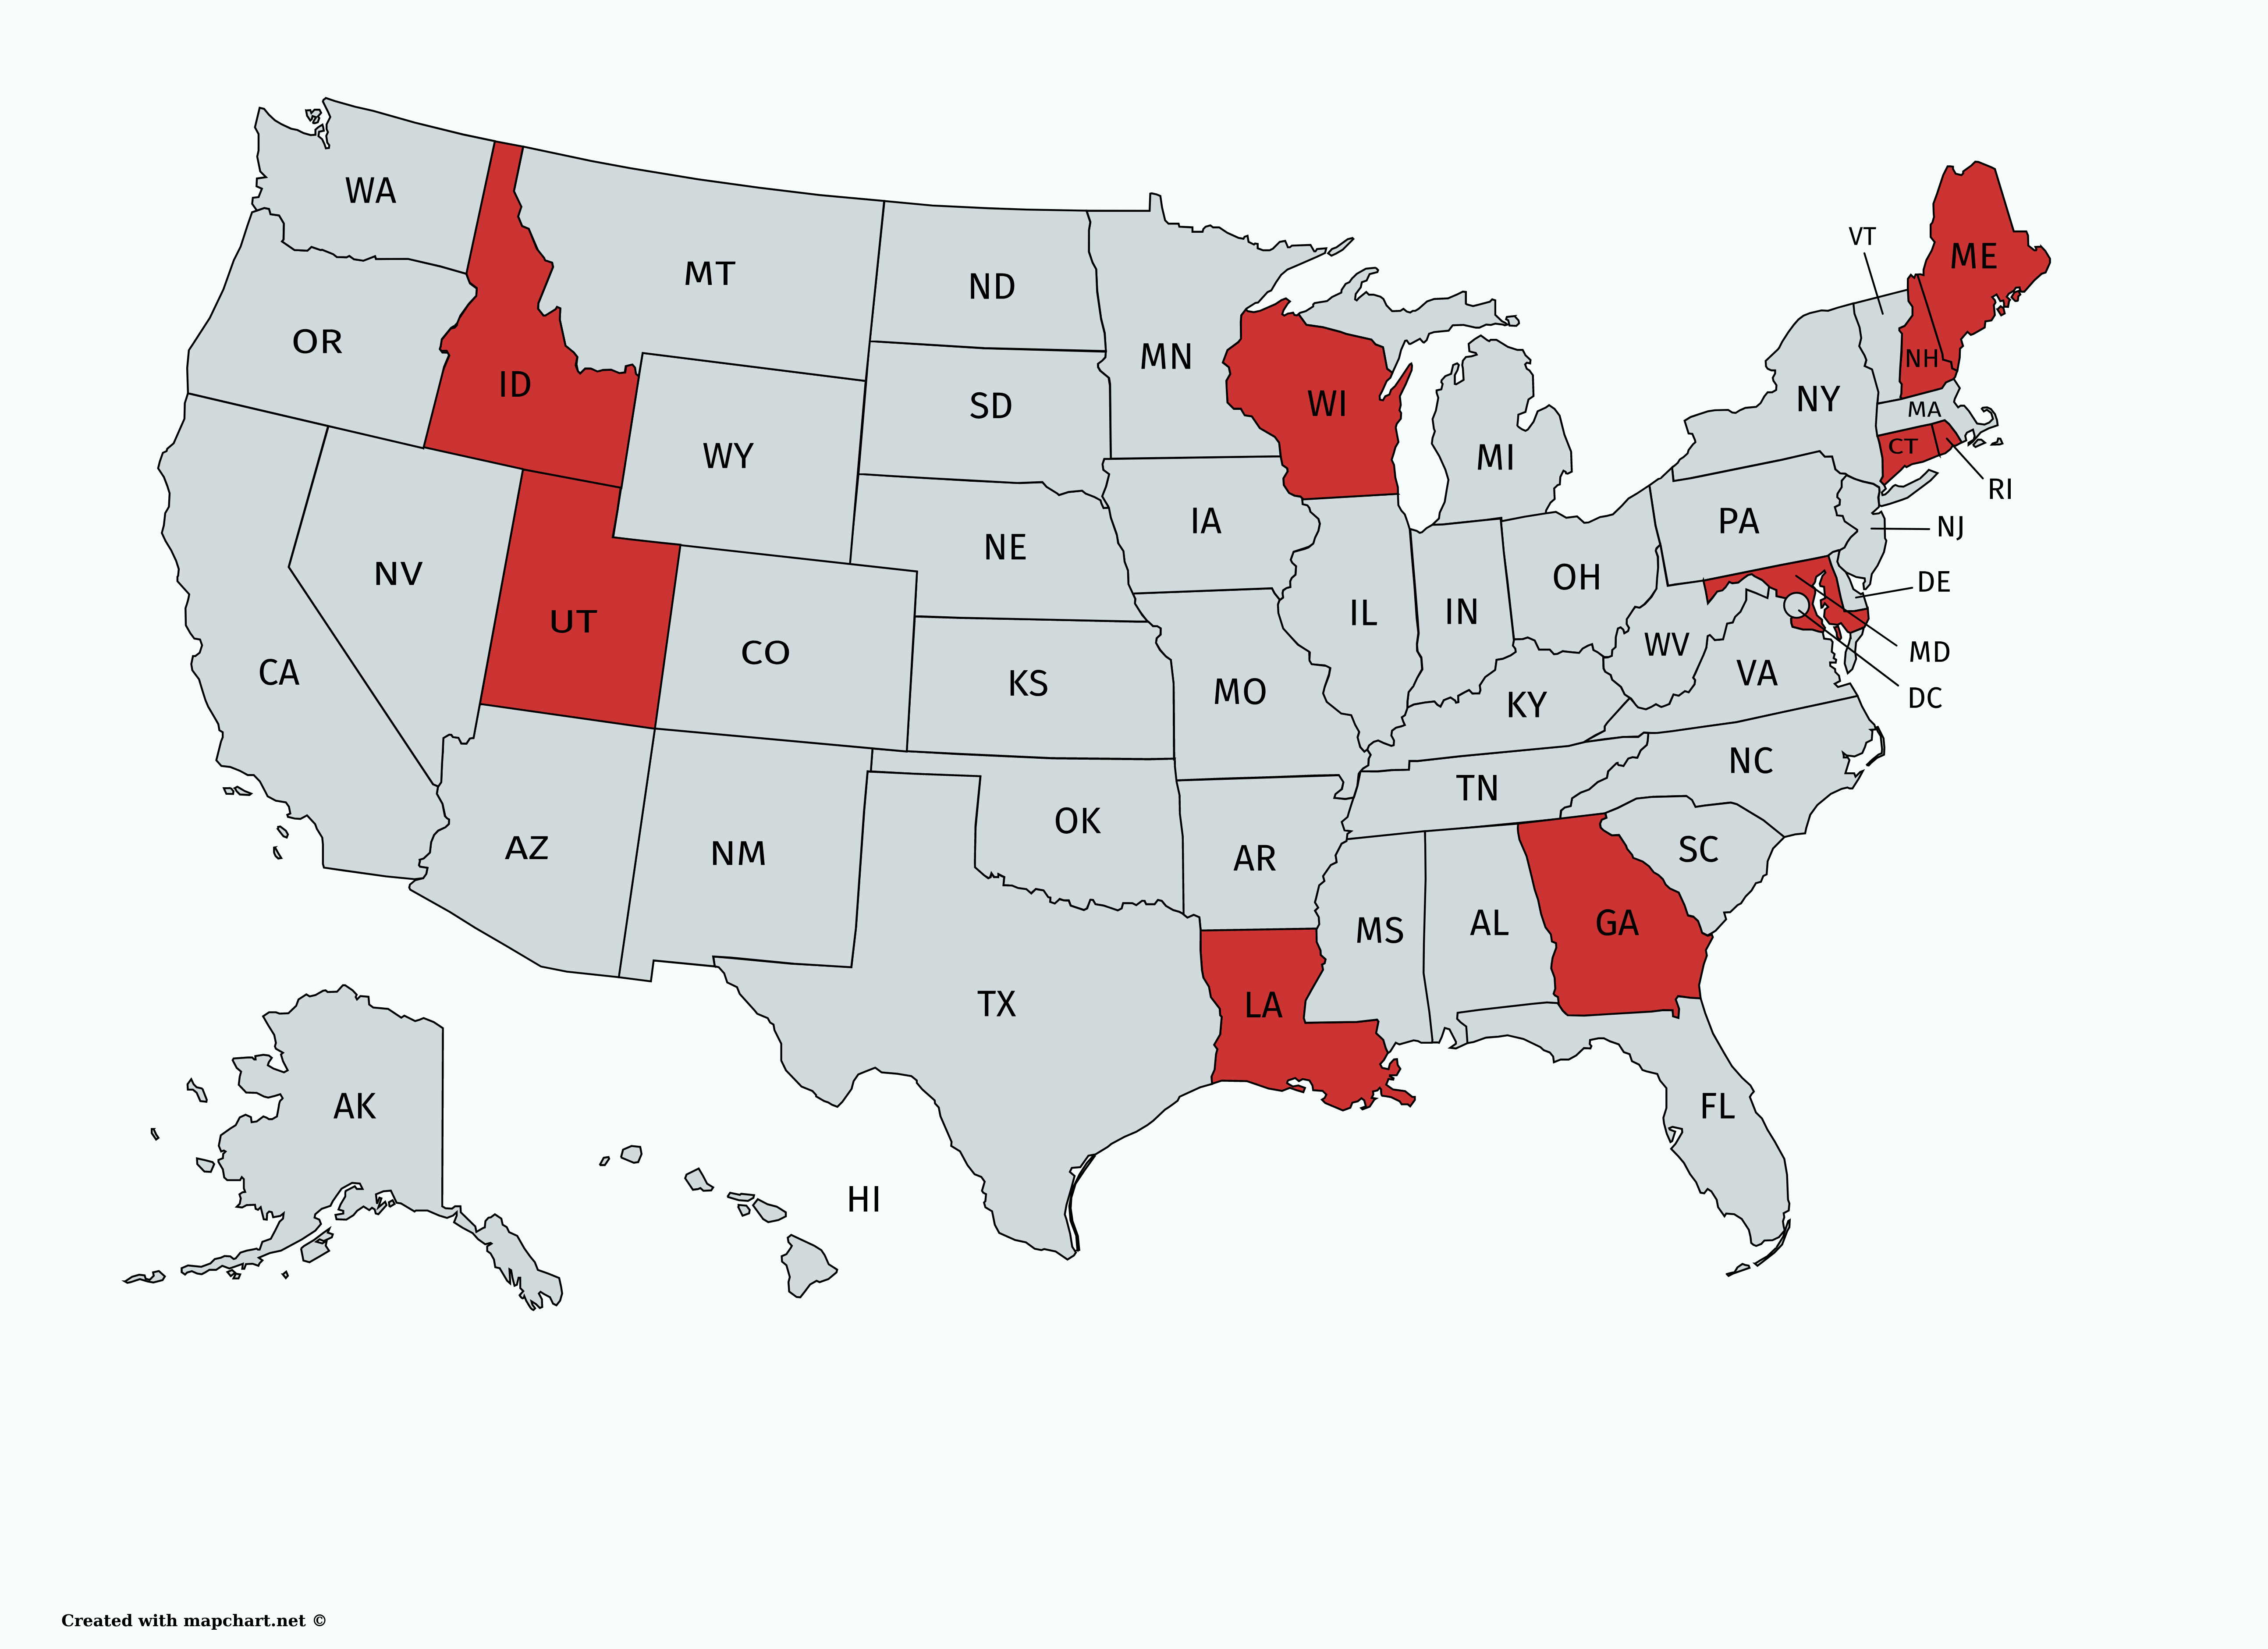
\includegraphics{./img/states_analysed.png}
\caption{States I analysed, marked in red \label{states_analysed}}
\end{figure}

Figure \ref{states_analysed} marks the states I analysed in red. I chose
these states mainly due to size considerations. All of these states are
small-to-medium sized (in terms of the number of Congressional
districts): the largest states like California, Texas and Florida are
absent. This is because my algorithm scales in both time and memory with
the \emph{square} of the size of the state (\(O(n^2)\)). The analysis is
achievable with larger desktop machines. Unfortunately, my own laptop
had only 8GB of RAM and not very much free disk space, making it
infeasible to examine larger states. Nonetheless, I was still able to
analyse medium-sized states like Louisiana, Maryland and Georgia (14
districts).

Size aside, I tried to get states that spanned the entire country,
including Western states (Idaho, Utah), Southern states (Louisiana,
Georgia), and Northeastern states (Maine, Rhode Island, New Hampshire,
Connecticut). I would also have liked to generate plans from a Pacific
state like Oregon and a Midwestern state like Kansas, but time
constraints prevented me from doing so.

Nonetheless, the number of states that I analyse exceeds most other
similar analyses. For instance, the seminal and heavily-cited work
\cite{cr2013} only analyse the state of Florida, and even very recent
work by \cite{ddj2019recom} and \cite{s2020} analyse only five and two
states respectively.

\hypertarget{calculating-spatial-diversity-and-compactness-scores-for-100000-plans}{%
\subsection{Calculating spatial diversity and compactness scores for
100,000
plans}\label{calculating-spatial-diversity-and-compactness-scores-for-100000-plans}}

After generating the plans, I calculate spatial diversity and
compactness scores for all of the plans. As mentioned, spatial diversity
is an operationalisation of district homogeneity: the higher spatial
diversity is, the less homogeneous (more heterogeneous) the district is.
I obtain data on spatial diversity from Professor Nicholas
Stephanopoulos. The dataset he gave me has eight \emph{factor scores}
for each Census Tract in the country, where a factor score is a combined
variable that covers vital areas like race, education, profession,
marital status, and housing. A district's spatial diversity score is
calculated by the sum of the standard deviation of each factor score,
normalised by the proportion of the variance each factor score explains.
As an example, consider a district made up of three Census Tracts (A, B,
C), and let each Tract have three factor scores (1, 2, 3). Let the
proportion of the variance explained by each factor score be 50\%, 30\%
and 20\% respectively. Then the total spatial diversity score would be:

\[ \sigma(A_1, B_1, C_1) \times 0.5 + \sigma(A_2, B_2, C_2) \times 0.3 + \sigma(A_3,
B_3, C_3) \times 0.2\]

I calculate spatial diversity score for every district, and, following
Stephanopoulos, take the arithmetic mean of all districts in a
districting plan to get the overall spatial diversity score for that
plan.

Next, I calculate compactness scores. As the Polsby-Popper metric is so
well-known and widely used, there was already an existing implementation
in the GerryChain library which I made use of. Similarly, existing
libraries like SciPy already had a Convex Hull method. Finally, I wrote
my own implementation of Reock, making use of the Smallest Enclosing
Circle code written by Project Nayuki \citep{nayuki2020}.

In order to calculate human compactness scores, I have to know where
voters live (to calculate driving durations between them). I therefore
obtain a dataset of ``voter representative points'' (VRPs) from
\cite{er2019}. These points aggregate many actual voters, downsampling
the data into a size that can be worked with. While this down-sampling
and placements of points randomly does introduce some noise, ``the
variability contributed\ldots{} is empirically very small''
\citep{er2019}. I sample 1,000 VRPs for each Congressional District in a
state. That means that a state like Maine with two districts will have
2,000 VRPs, and a state like Louisiana---with seven districts before the
new redistricting plan---will have 7,000.

I then calculate all pairwise driving durations between all VRPs using
an open-source routing engine called Open Source Routing Machine (OSRM)
built by \cite{osrm}. The routing engine is able to calculate driving
durations between any two points---very similar to Google Maps---but the
number of queries it can process is orders of magnitude larger than the
limits imposed by the Google Maps API. For these ten states, I calculate
about 400 million point-to-point driving durations in total. As point of
comparison, using Google Map's
\href{https://developers.google.com/maps/documentation/distance-matrix/usage-and-billing}{Distance
Matrix API} for that number of requests would cost \$1,480,000\footnote{Volume
  discounts do exist, but you have to contact the Sales Team, and I
  doubt I could afford it anyway\ldots{}}. And if I had tried to analyse
California (with 53 Congressional districts), this would require almost
3 billion point-to-point driving durations.

Because my analysis is on the tract level, I map VRPs to Census Tracts
using a spatial join. I sum the pairwise point-to-point distances to get
a matrix of pairwise \emph{tract-to-tract} driving durations. I then sum
the driving durations from each point in the district to another and
calculate the human compactness score for each district.

Finally, I aggregate the individual district scores into a plan-level
score by simply taking the arithmetic mean. For instance, if a
districting plan has three districts with Polsby-Popper scores of 0.25,
0.5, and 1, the Polsby-Popper score for that plan would be
\((0.25 + 0.5 + 1) / 3 = 0.5833\). As a robustness check, I also use the
sum of square roots as an aggregation function: that is,
\(\sqrt{0.25} + \sqrt{0.5} + \sqrt{1} = 0.736\)\footnote{This penalises
  districting plans that have a large difference between districts
  e.g.~one very good district and one very bad one.}, obtaining
qualitatively similar results.

\hypertarget{performing-data-analysis-on-the-100000-plans}{%
\subsection{Performing data analysis on the 100,000
plans}\label{performing-data-analysis-on-the-100000-plans}}

After calculating the overall spatial diversity and compactness scores
on all the plans, I start running exploratory data analysis and
statistical tests. The results are detailed below.

\hypertarget{results}{%
\section{Results}\label{results}}

{[}TODO{]} take andys comments

My key results are as follows:

\begin{enumerate}
\def\labelenumi{\arabic{enumi}.}
\item
  The choice of compactness measure can result in very different plans
\item
\end{enumerate}

Comparing different compactness measures, I

\begin{enumerate}
\def\labelenumi{\arabic{enumi}.}
\setcounter{enumi}{2}
\tightlist
\item
  Different compactness measures are correlated with one
  another\footnote{The geometric compactness measures agree most with
    one another, the human compactness measure not as much.}.
\item
  Only human compactness is negatively correlated with spatial
  diversity: geometric/dispersion-based measures have either no or a
  positive (bad) effect on spatial diversity\footnote{OLS regressions
    with state dummies show that only human compactness has a
    significantly negative coefficient on spatial diversity.
    Difference-in-means tests show that only the most compact plans
    under human compactness are less spatially diverse than average, and
    are less spatially diverse than the most compact plans under
    geometric/dispersion-based measures.}.
\end{enumerate}

Overall, the evidence suggests that optimising over compactness will
give you less spatially diverse districts, and human compactness will do
the best job of it.

\hypertarget{initial-analysis}{%
\subsection{Initial analysis}\label{initial-analysis}}

Before proceeding to the quantitative statistical tests that answer my
main research question, I want to do a bit of preliminary analysis to
show what the generated plans look like and what the \emph{distribution}
of those plans looks like. This will help us contextualise the key
results that come next. I also present some interesting supplementary
results that largely accord with our intuitions.

\hypertarget{the-choice-of-compactness-measure-can-result-in-very-different-plans}{%
\subsubsection{The choice of compactness measure can result in very
different
plans}\label{the-choice-of-compactness-measure-can-result-in-very-different-plans}}

After having obtained all the plans and their corresponding scores, I
plot the plans with the best and worst spatial diversity and compactness
scores to get an understanding for the types of plans that each metric
encourages. This will give us valuable intuition for understanding the
subsequent results.

For ease of exposition I show states with only two districts, but the
analysis extends to states with any number of districts. (Plots of the
other eight states are available in my GitHub repository). I also use
Polsby-Popper to represent the other two dispersion-based compactness
metrics as my explanations are similarly applicable to those metrics.

\begin{figure}
\centering
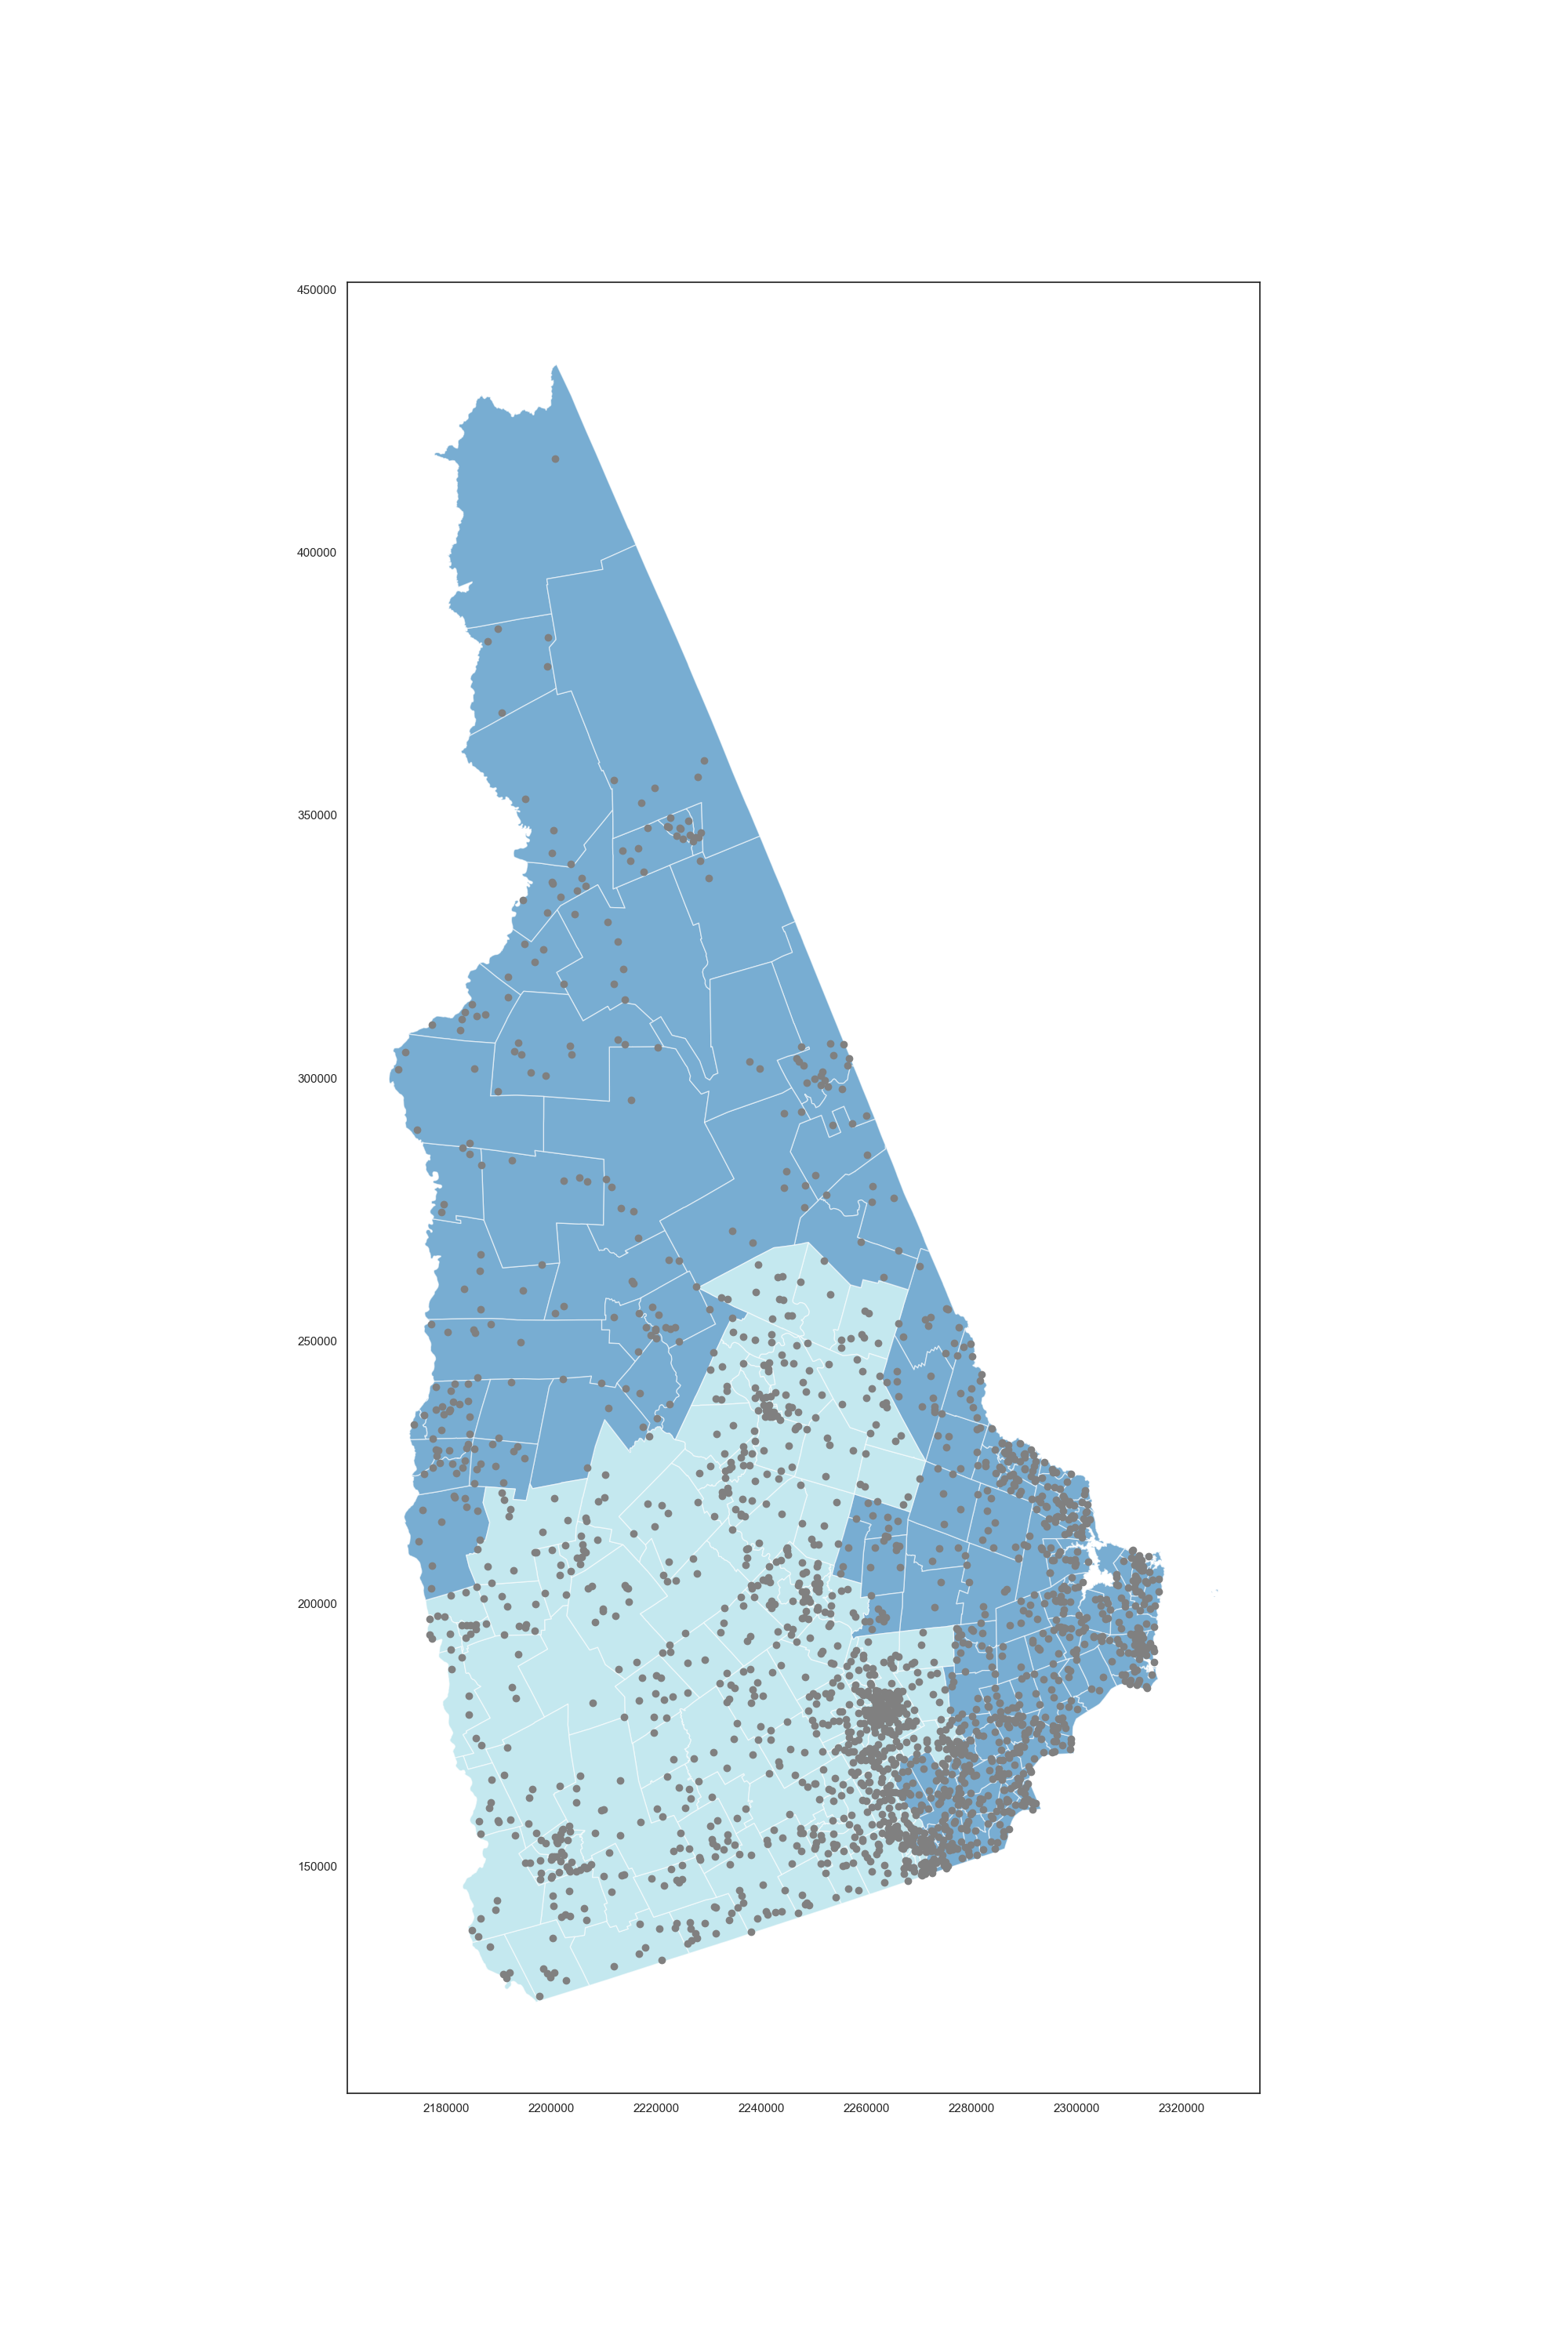
\includegraphics{../30_results/33_points_on_tracts.png}
\caption{Population density plot of New Hampshire. Each dot represents
roughly 600 people. \label{nh_density}}
\end{figure}

\begin{figure}
\centering
\includegraphics{../30_results/33_min_max_subplots.png}
\caption{Best and worst districting plans of New Hampshire under
different metrics \label{nh_minmax}}
\end{figure}

Figure \ref{nh_minmax} plots the best and worst plans according to
several metrics. Let us begin with the middle row (Polsby-Popper), as
its interpretation is the most straightforward. The Polsby-Popper (and
other dispersion-based) metric penalises districts that are very
``snakelike'' and prefers districts that have regular shapes like
squares or circles. This is clearly reflected in the plot. The best plan
has a district with a very regular shape, and the worst plan has a
snakelike district that contorts through half the state.

On the top row is human compactness. A good plan under human compactness
minimises the total travel times between every member of the district.
This encourages small, compact districts that avoid splitting urban
centers.

We can see that the top plan under human compactness corresponds well to
the actual population density of New Hampshire as seen in Figure
\ref{nh_density}. The top plan puts the two most populous and urban
counties in New Hampshire---Rockingham and Hillsborough---together in
the same district. The worst plan under human compactness splits the
counties in such a way that one's co-districtors are far away, and one's
nearest neighbours are in a separate district.

As expected, the top plan under spatial diversity (bottom row) closely
resembles the top plan under human compactness. In relatively
homogeneous New Hampshire, the main source of spatial diversity is the
urban-rural divide. A plan that keeps urbanites together in one district
is favoured under spatial diversity.

And while the worst plan under spatial diversity looks different from
that under human compactness at first glance, they are actually quite
similar. Both plans split up the two populous urban counties, having a
``fish-hook'' shaped district that starts from the rural north of the
state and swoops down to the south to carve out a large part of the
counties.

This case study shows that dispersion-based measures may not always
reflect existing communities of interest. This seems to fuel criticism
of dispersion-based measures on exactly that basis (``it makes no sense
to combine areas that have nothing in common except that they fit neatly
into a square'' \citep{wolf2015}). In this example, human compactness
and spatial diversity agree neatly on what the best districting plans
should look like.

While human compactness generally tracks spatial diversity better than
other compactness metrics (I provide evidence for this later), it does
not always do so. Figure \ref{idaho_density} gives the population of
Idaho. We can see that a large proportion of the population is
concentrated in a U-shaped ``belt'' spanning the southern half of the
state. A good plan under spatial diversity will attempt to put this
relatively urban ``belt'' in the same district, and this is indeed what
we observe in Figure \ref{idaho_minmax}. But due to its great distance
and jagged perimeter, such a plan is penalised under both human
compactness and dispersion-based measures, both of which prefer a
relatively compact square-shaped district.

\begin{figure}
\centering
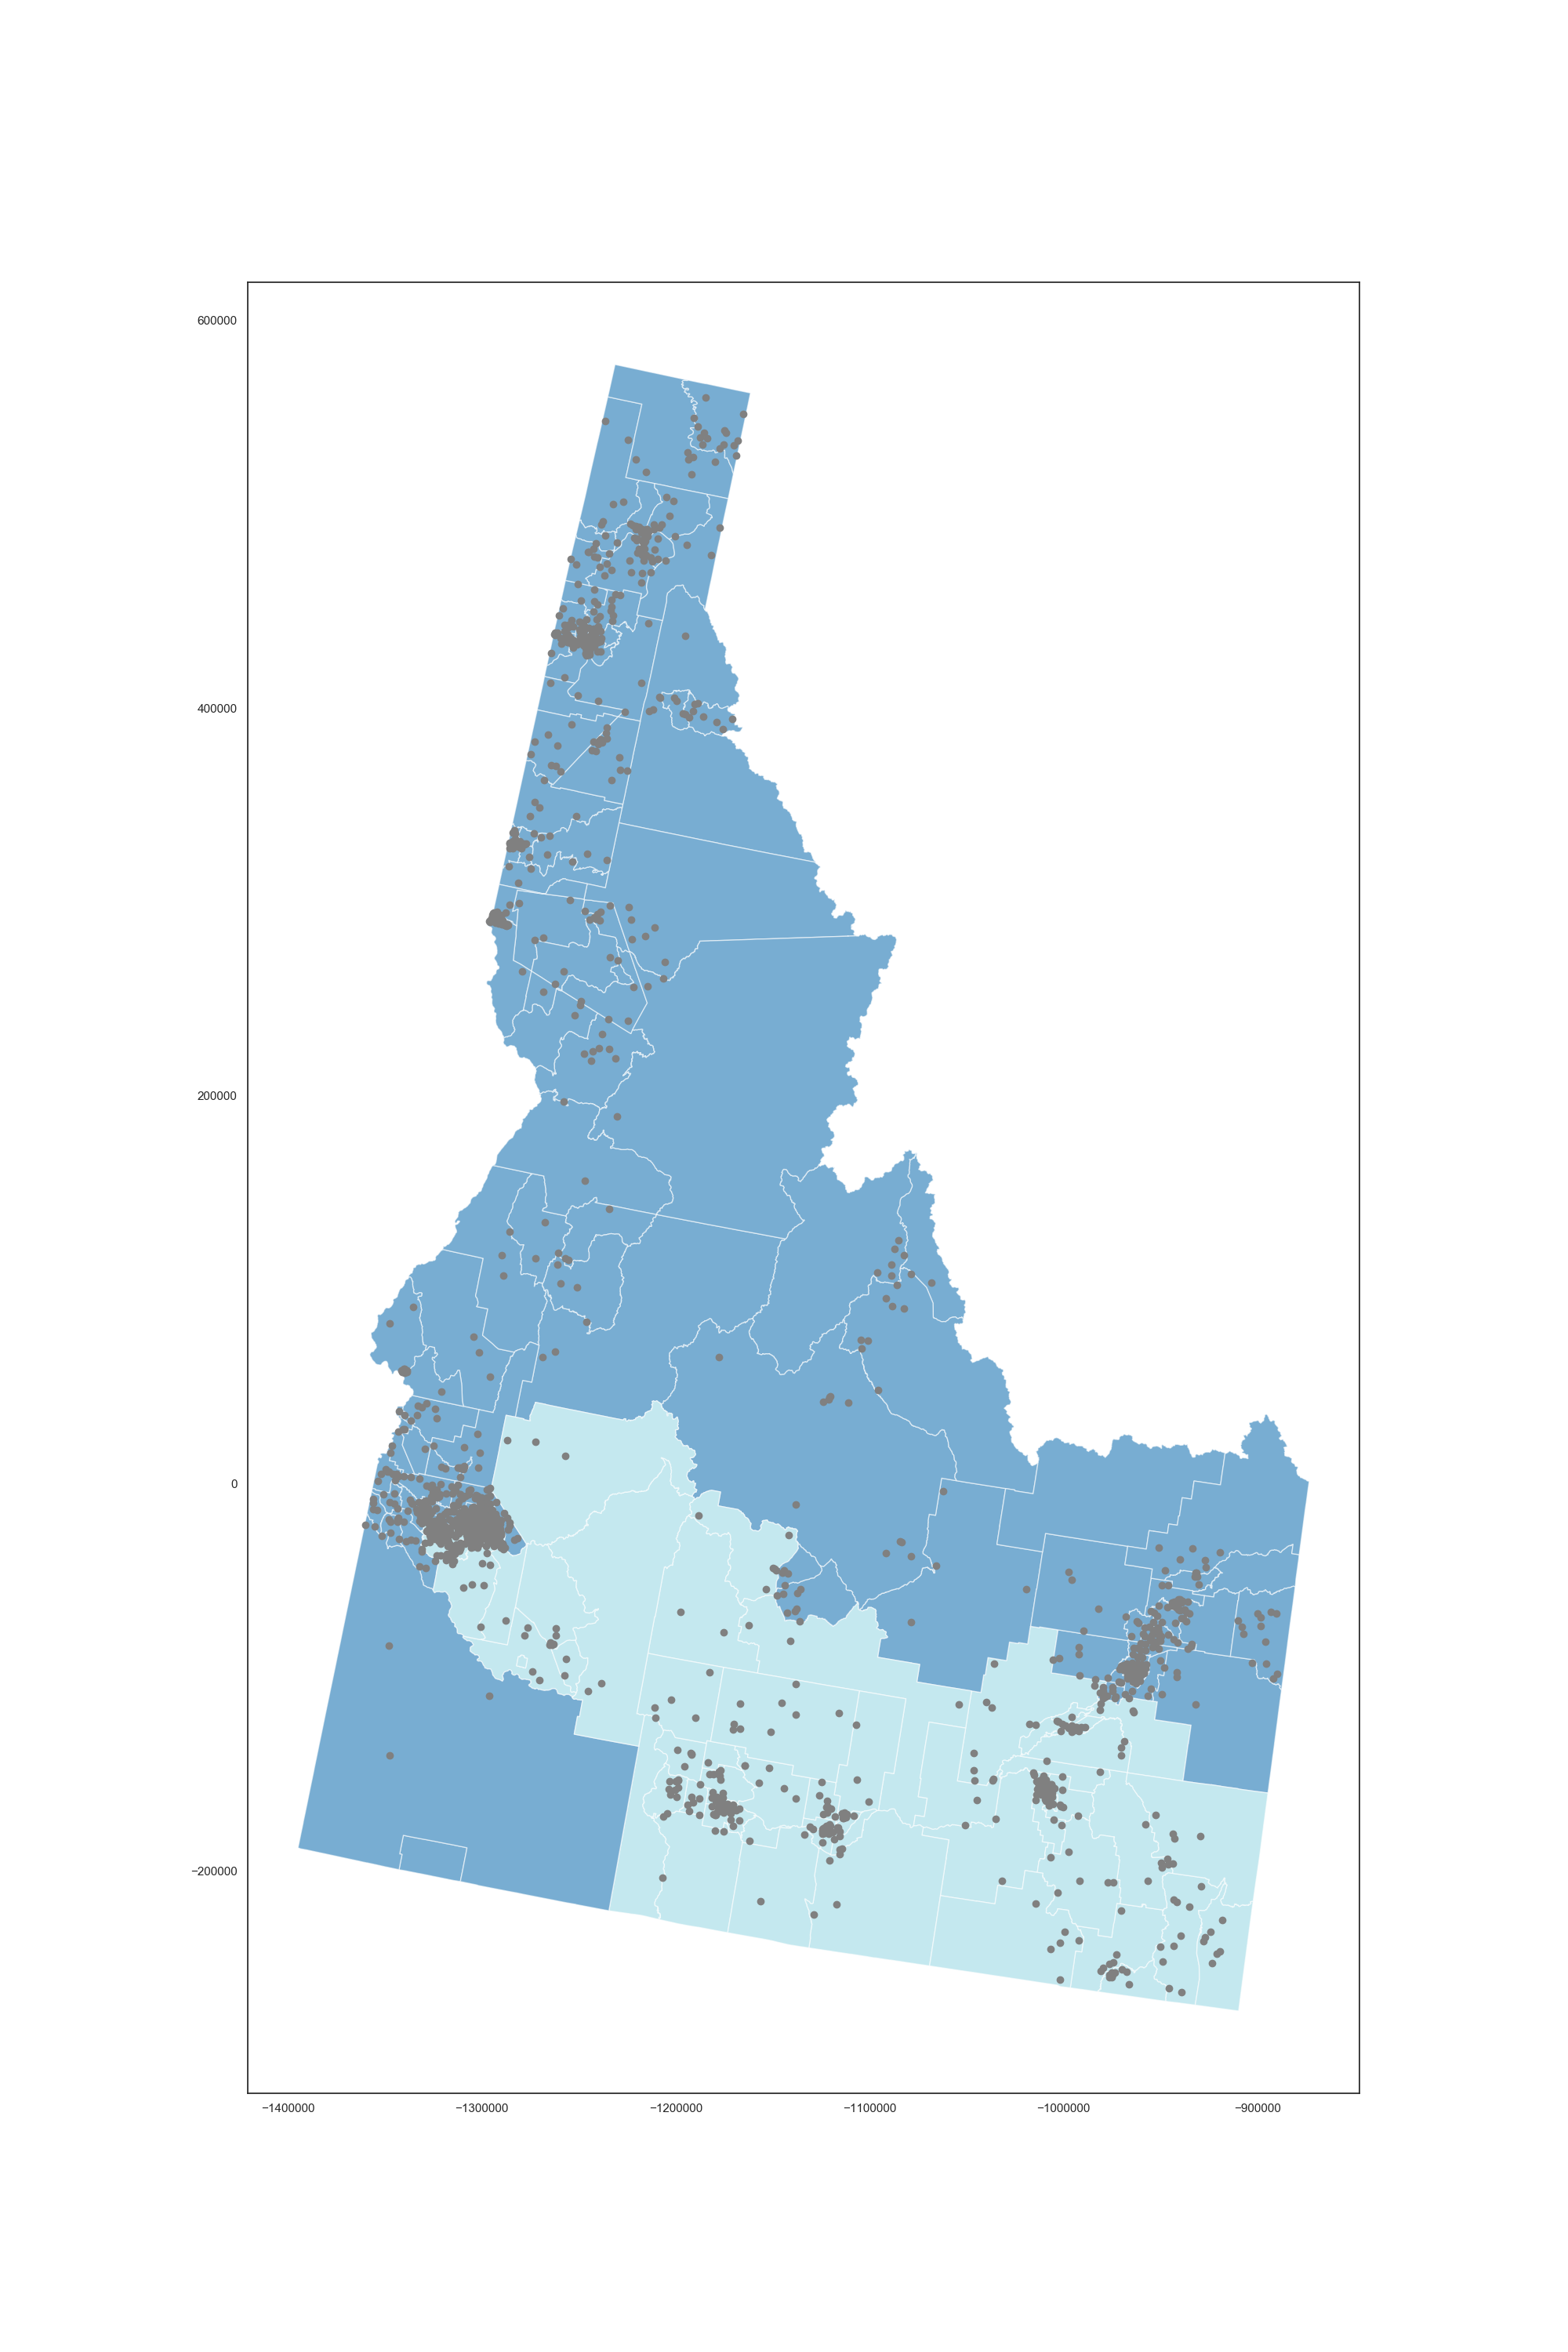
\includegraphics{../30_results/16_points_on_tracts.png}
\caption{Population density plot of Idaho. Each point represents
\textasciitilde{}700 people. \label{idaho_density}}
\end{figure}

\begin{figure}
\centering
\includegraphics{../30_results/16_min_max_subplots.png}
\caption{Best and worst districting plans of Idaho under different
metrics \label{idaho_minmax}}
\end{figure}

As we can see, compactness measures need not always agree with spatial
diversity, particularly in the case study of Idaho. Intuitively, this
seems to make sense: spatial diversity tries to put similar people
together, and people who live in the same area are often, but not
always, similar. It is also encouraging that the difference compactness

\hypertarget{compactness-measures-largely-agree-with-one-another-but-human-compactness-less-so}{%
\subsubsection{Compactness measures largely agree with one another, but
human compactness less
so}\label{compactness-measures-largely-agree-with-one-another-but-human-compactness-less-so}}

Despite the fact that compactness measures can result in radically
different-looking plans, as shown in the previous section, compactness
measures largely agree with one another. By looking at the correlations
between different compactness measures, I find that a plan that scores
highly on one compactness metric will likely score highly on another.
The correlations are strongest between the three geometric compactness
measures, and lower (but still significantly positive) between the
geometric and human compactness measures.

One way to visualise these correlations is through the use of a heatmap.
Figure \ref{connecticut_corr} plots the correlation coefficients between
each pair of metrics. Firstly, we can see the correlation coefficients
between spatial diversity (sd) and the compactness metrics. Here, it
seems like human compactness has a significant negative correlation with
spatial diversity, with the other compactness metrics having little
correlation. We can also see that the correlation between human
compactness and geometric compactness measures are somewhat lower
(\textasciitilde{}0.46) than the correlations between different
geometric measures. I made a point not to aggregate all the observations
from each state into a pooled data set, because looking at the aggregate
results can be highly misleading if there is a single outlier state that
biases the results.

\begin{figure}
\centering
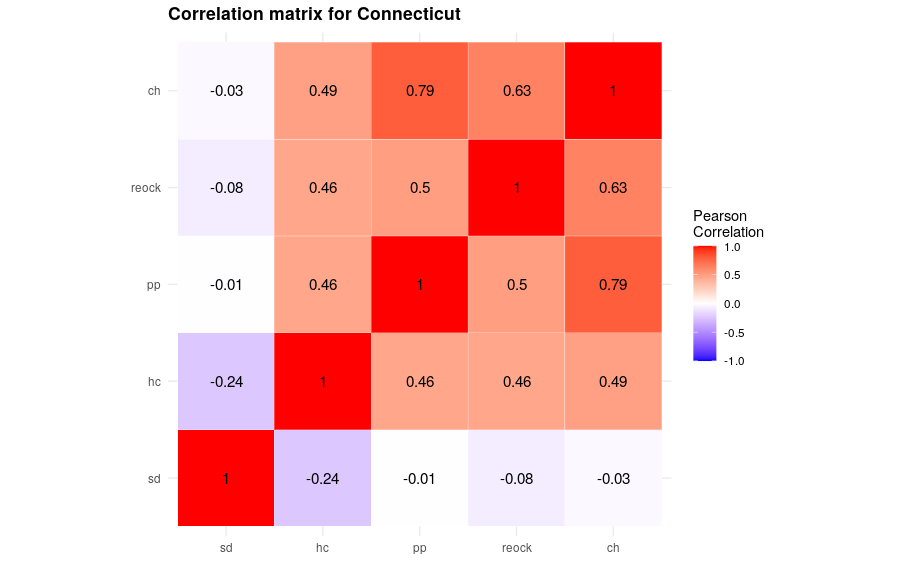
\includegraphics{../30_results/corr_matrix_connecticut.png}
\caption{Correlation heatmap of Connecticut \label{connecticut_corr}}
\end{figure}

This finding is somewhat surprising and nonobvious. We would expect the
different geometric compactness measures to track each other very
closely as they are measuring very similar things. It is much less
obvious, however, that purely geometric measures would agree with a
metric that measures driving durations between points. This result is
encouraging because it shows that these metrics are able to get at the
same concept of compactness despite having completely different
theoretical backgrounds.

While the compactness measures largely agree with each other in most of
the states, they are not unanimous. The correlation heatmap of Utah
shows a case where human compactness and the other geometric measures
disagree. Here, the correlation between geometric compactness measures
is very high (0.89---almost 1), but there is in fact a negative
correlation between human compactness and the geometric measures.

\begin{figure}
\centering
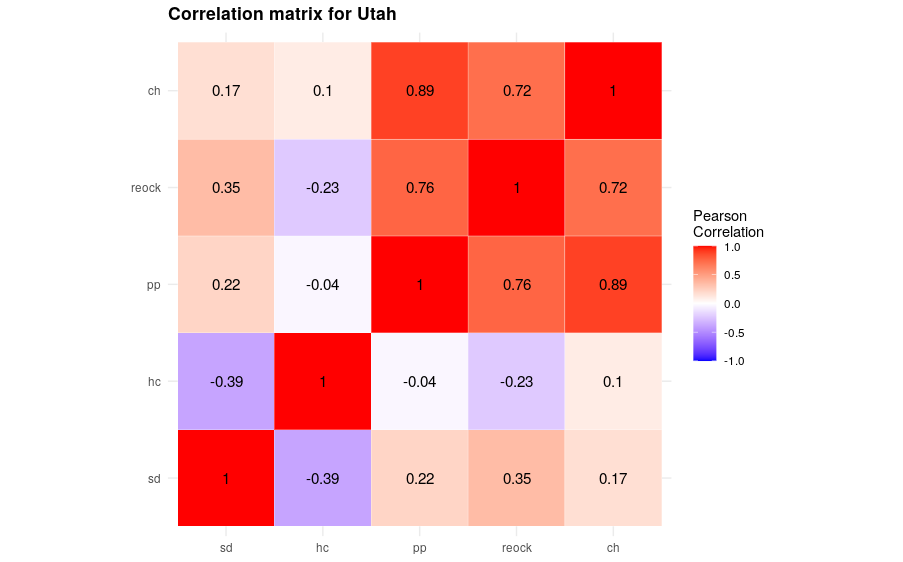
\includegraphics{../30_results/corr_matrix_utah.png}
\caption{Correlation heatmap of Utah}
\end{figure}

These results vindicate my choice to use an ensemble of compactness
metrics rather than relying on a single measure. While the correlation
between metrics is high, it is not perfect, and indeed we observe cases
like Utah where the compactness measures disagree.

\hypertarget{robustness-check}{%
\paragraph{Robustness check}\label{robustness-check}}

As a robustness check, I have also visualised the findings through
pairwise scatterplots. These plots have the advantage of being able to
visualise the scatterplots, which can surface non-linear relationships
that a simple correlation coefficient cannot. The pairwise scatterplots
show that the relationship between compactness metrics is always linear.
As an example, Figure \ref{pairwise_plot_grouped} shows an example
correlation plot between spatial diversity and the various compactness
metrics for the state of Georgia. I have included correlation matrices
and pairwise scatterplots for all ten states in my GitHub repository.
They confirm that the overall correlation is positive for most states,
with human compactness being less correlated overall with the other
metrics.

\begin{figure}
\centering
\includegraphics{../30_results/13_pairwise_plot_grouped.png}
\caption{Correlation plot of Georgia\label{pairwise_plot_grouped}}
\end{figure}

\hypertarget{spatial-diversity-varies-a-lot-between-states-but-little-within-states}{%
\subsubsection{Spatial diversity varies a lot between states but little
within
states}\label{spatial-diversity-varies-a-lot-between-states-but-little-within-states}}

Each state occupies a narrow band in the range of possible spatial
diversity scores. While spatial diversity scores of the districting
plans of the ten states I examine range from 0.50 to 0.80, districting
plans in a state vary by only around 0.05, as can be observed in Figure
\ref{sd_plans}.

\begin{figure}
\centering
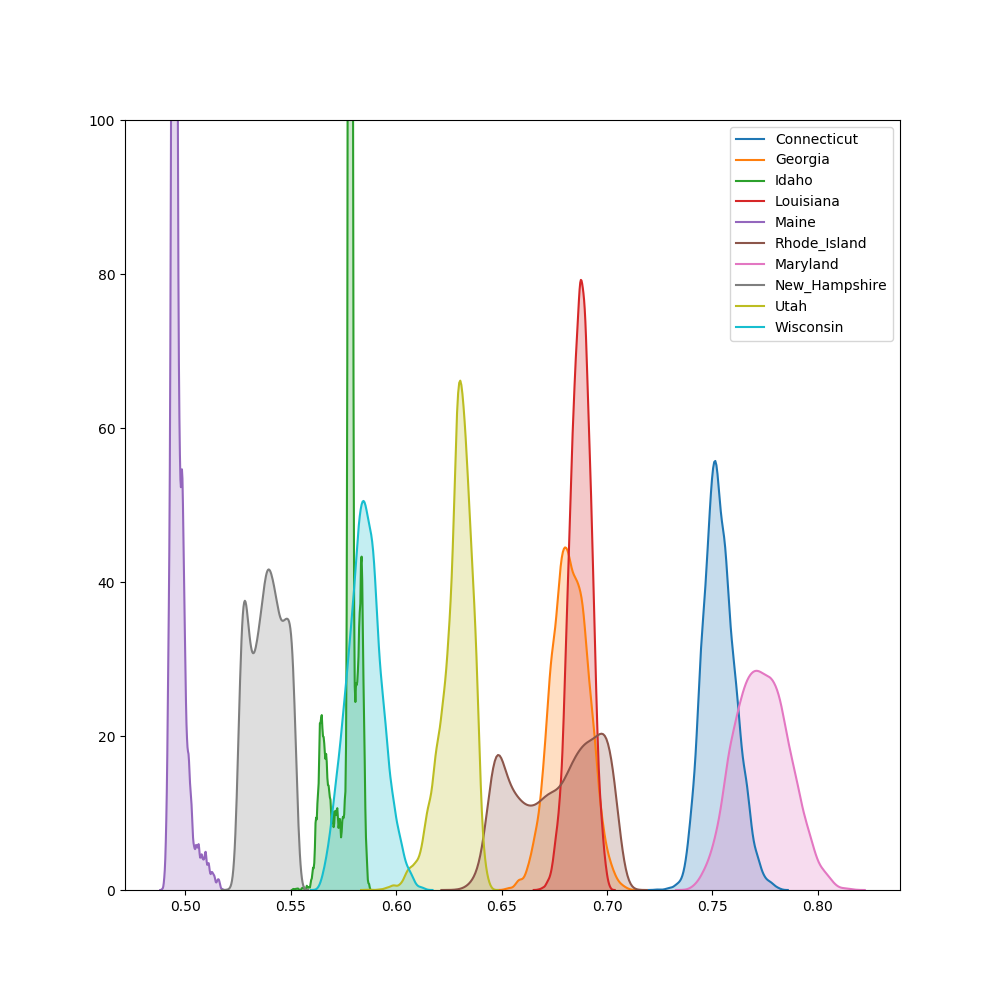
\includegraphics{../30_results/all_plans_sd.png}
\caption{Overall spatial diversity of districting plans by state
\label{sd_plans}}
\end{figure}

Figure \ref{sd_plans} plots While this range is small, it is not
insignificant: Figure \ref{sd_responsiveness} shows that an increase in
a state's spatial diversity by 0.05 is correlated with a decrease in
electoral responsiveness by 0.3, about 10\% of the variance.

\hypertarget{small-urban-districts-are-usually-more-spatially-diverse}{%
\subsubsection{Small urban districts are usually more spatially
diverse}\label{small-urban-districts-are-usually-more-spatially-diverse}}

One finding consistent across all states is that the smaller (by area)
the district, the higher the spatial diversity. Figure
\ref{pairwise_plot} is a density plot of districts binned by area. The
x-axis gives the spatial diversity score and the y-axis gives how many
districts in the 10,000 plans had that spatial diversity score.

\begin{figure}
\centering
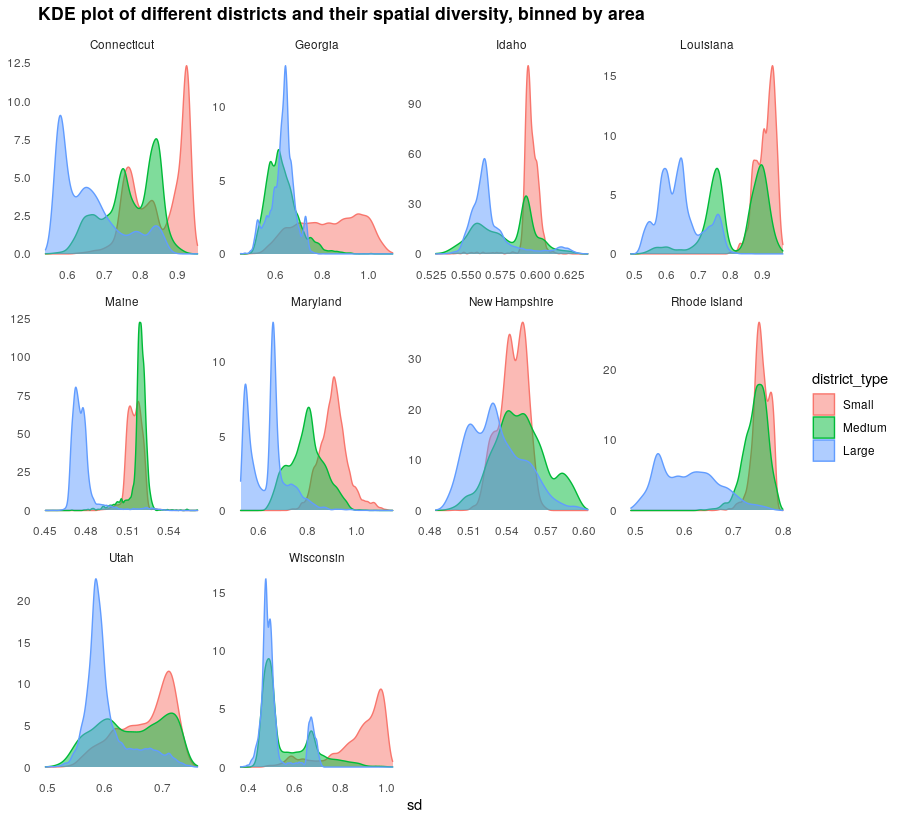
\includegraphics{../30_results/size_and_sd.png}
\caption{Small urban districts (in red) are the most heterogeneous
\label{pairwise_plot}}
\end{figure}

We can see that large districts (in blue) tend to occupy the low end of
the spatial diversity range, with medium-sized districts (green) in the
middle, and the smallest districts (in red) have the highest spatial
diversity. This finding is quite intuitive. Cities tend to be the most
heterogeneous parts of a state, with people of different races, ages,
and socioeconomic classes. This suggests that more urban states will
simply have larger spatial diversity scores, which helps to explain why
spatial diversity varies greatly between plans of different states but
little within plans of the same state.

\hypertarget{conclusions-of-initial-data-exploration}{%
\subsubsection{Conclusions of initial data
exploration}\label{conclusions-of-initial-data-exploration}}

We have seen that the overall distribution of districting plans per
state lie within a tight bound, largely determined by each state's
political geography. This suggests that while districting can exert an
effect on political outcomes, we should not expect optimising for
compactness to change spatial diversity very much in a representative
subset of plans drawn by a nonpartisan districting committee.

We have also seen that

\hypertarget{key-results}{%
\subsection{Key results}\label{key-results}}

{[}TODO{]}

Having completed the preliminary analyses, we can now move to the key
results of my analysis. How do different compactness measures compare
with one another, and is there a trade-off between compactness and
communities of interest? The evidence suggests that some compactness
measures may \ldots{}

\hypertarget{only-human-compactness-positively-correlates-with-district-homogeneity}{%
\subsubsection{Only human compactness positively correlates with
district
homogeneity}\label{only-human-compactness-positively-correlates-with-district-homogeneity}}

Next, I run multivariate OLS regressions with country dummies and
difference-in-means tests, and find no significant effects of geometric
compactness on spatial diversity. I find that human compactness has a
significant negative effect on spatial diversity: increasing human
compactness from 0 to 1 decreases spatial diversity by 0.04 points.

We cannot simply run a regression aggregating every single district as
each state has a unique distribution of spatial diversity and
compactness. Consider the following. Within each state, increasing
compactness decreases spatial diversity. But on the aggregate, states
with high spatial diversity also have low compactness. In this case,
regressing spatial diversity on the aggregate level would give an
inflated estimate of the actual effect, falling afoul of the
\emph{ecological fallacy}. I illustrate this in figures \ref{indiv_reg}
and \ref{grouped_reg}. In Figure \ref{indiv_reg}, I plot a graph of
human compactness on the x-axis and spatial diversity on the y-axis. The
overall trend seems to be slightly negative: in most of the groups,
there is a slight negative correlation between human compactness and
spatial diversity. However, we would obtain erroneous results if we
aggregated the different states and ran a singular regression. This is
depicted in Figure \ref{grouped_reg}: due to the \emph{between-group}
correlation of compactness and spatial diversity, the estimate of the
effect is biased.

\begin{figure}
\centering
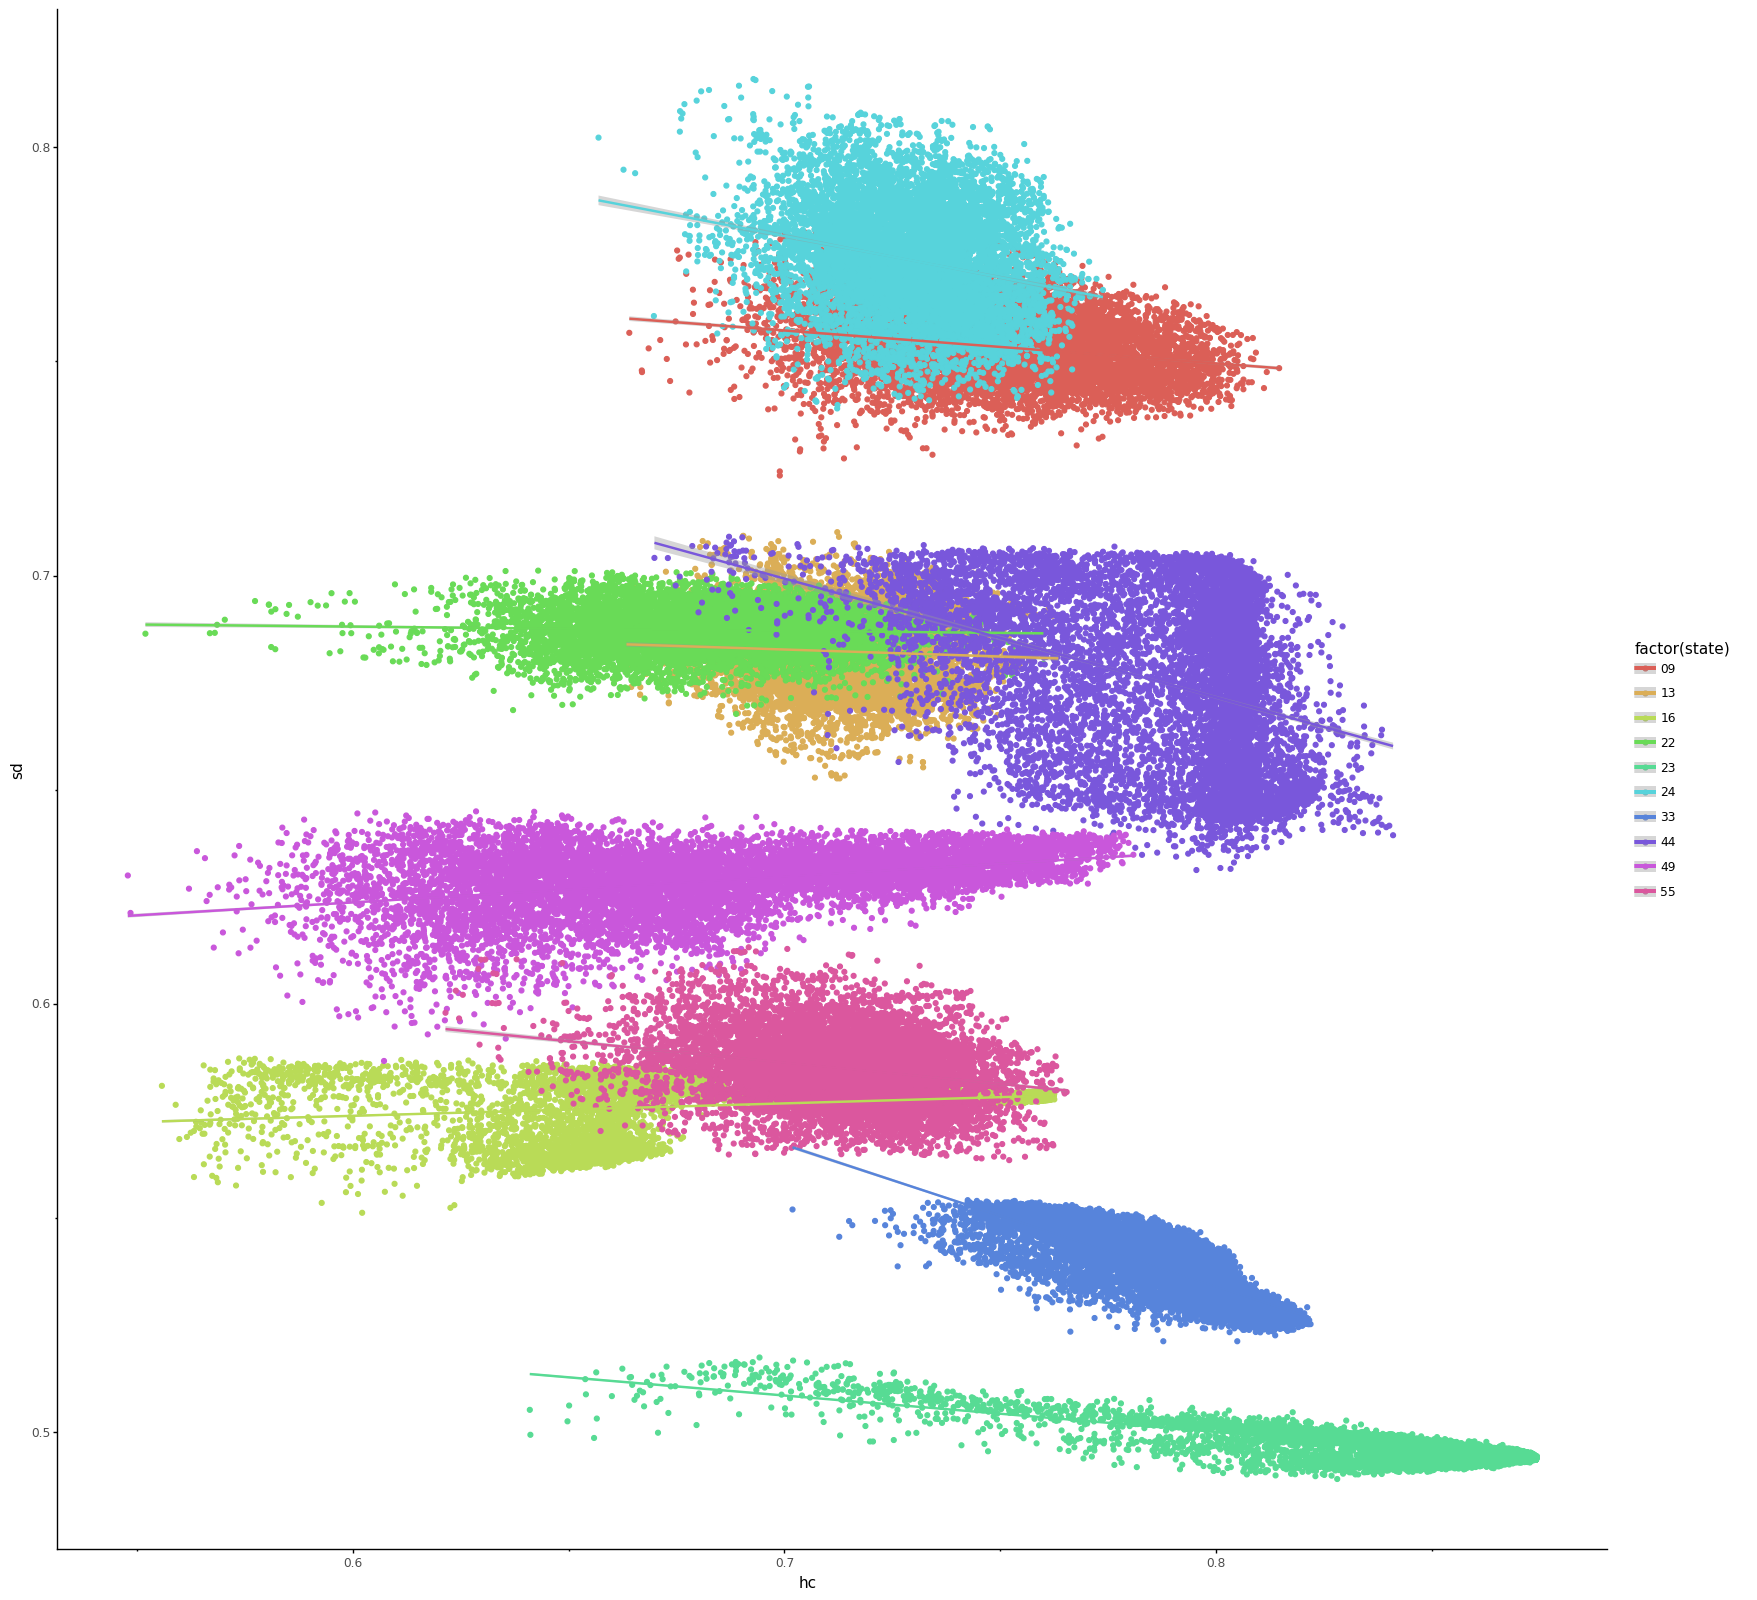
\includegraphics{../30_results/individual_regressions.png}
\caption{The individual-level regressions show a weak negative
correlation between human compactness and spatial
diversity\label{indiv_reg}}
\end{figure}

\begin{figure}
\centering
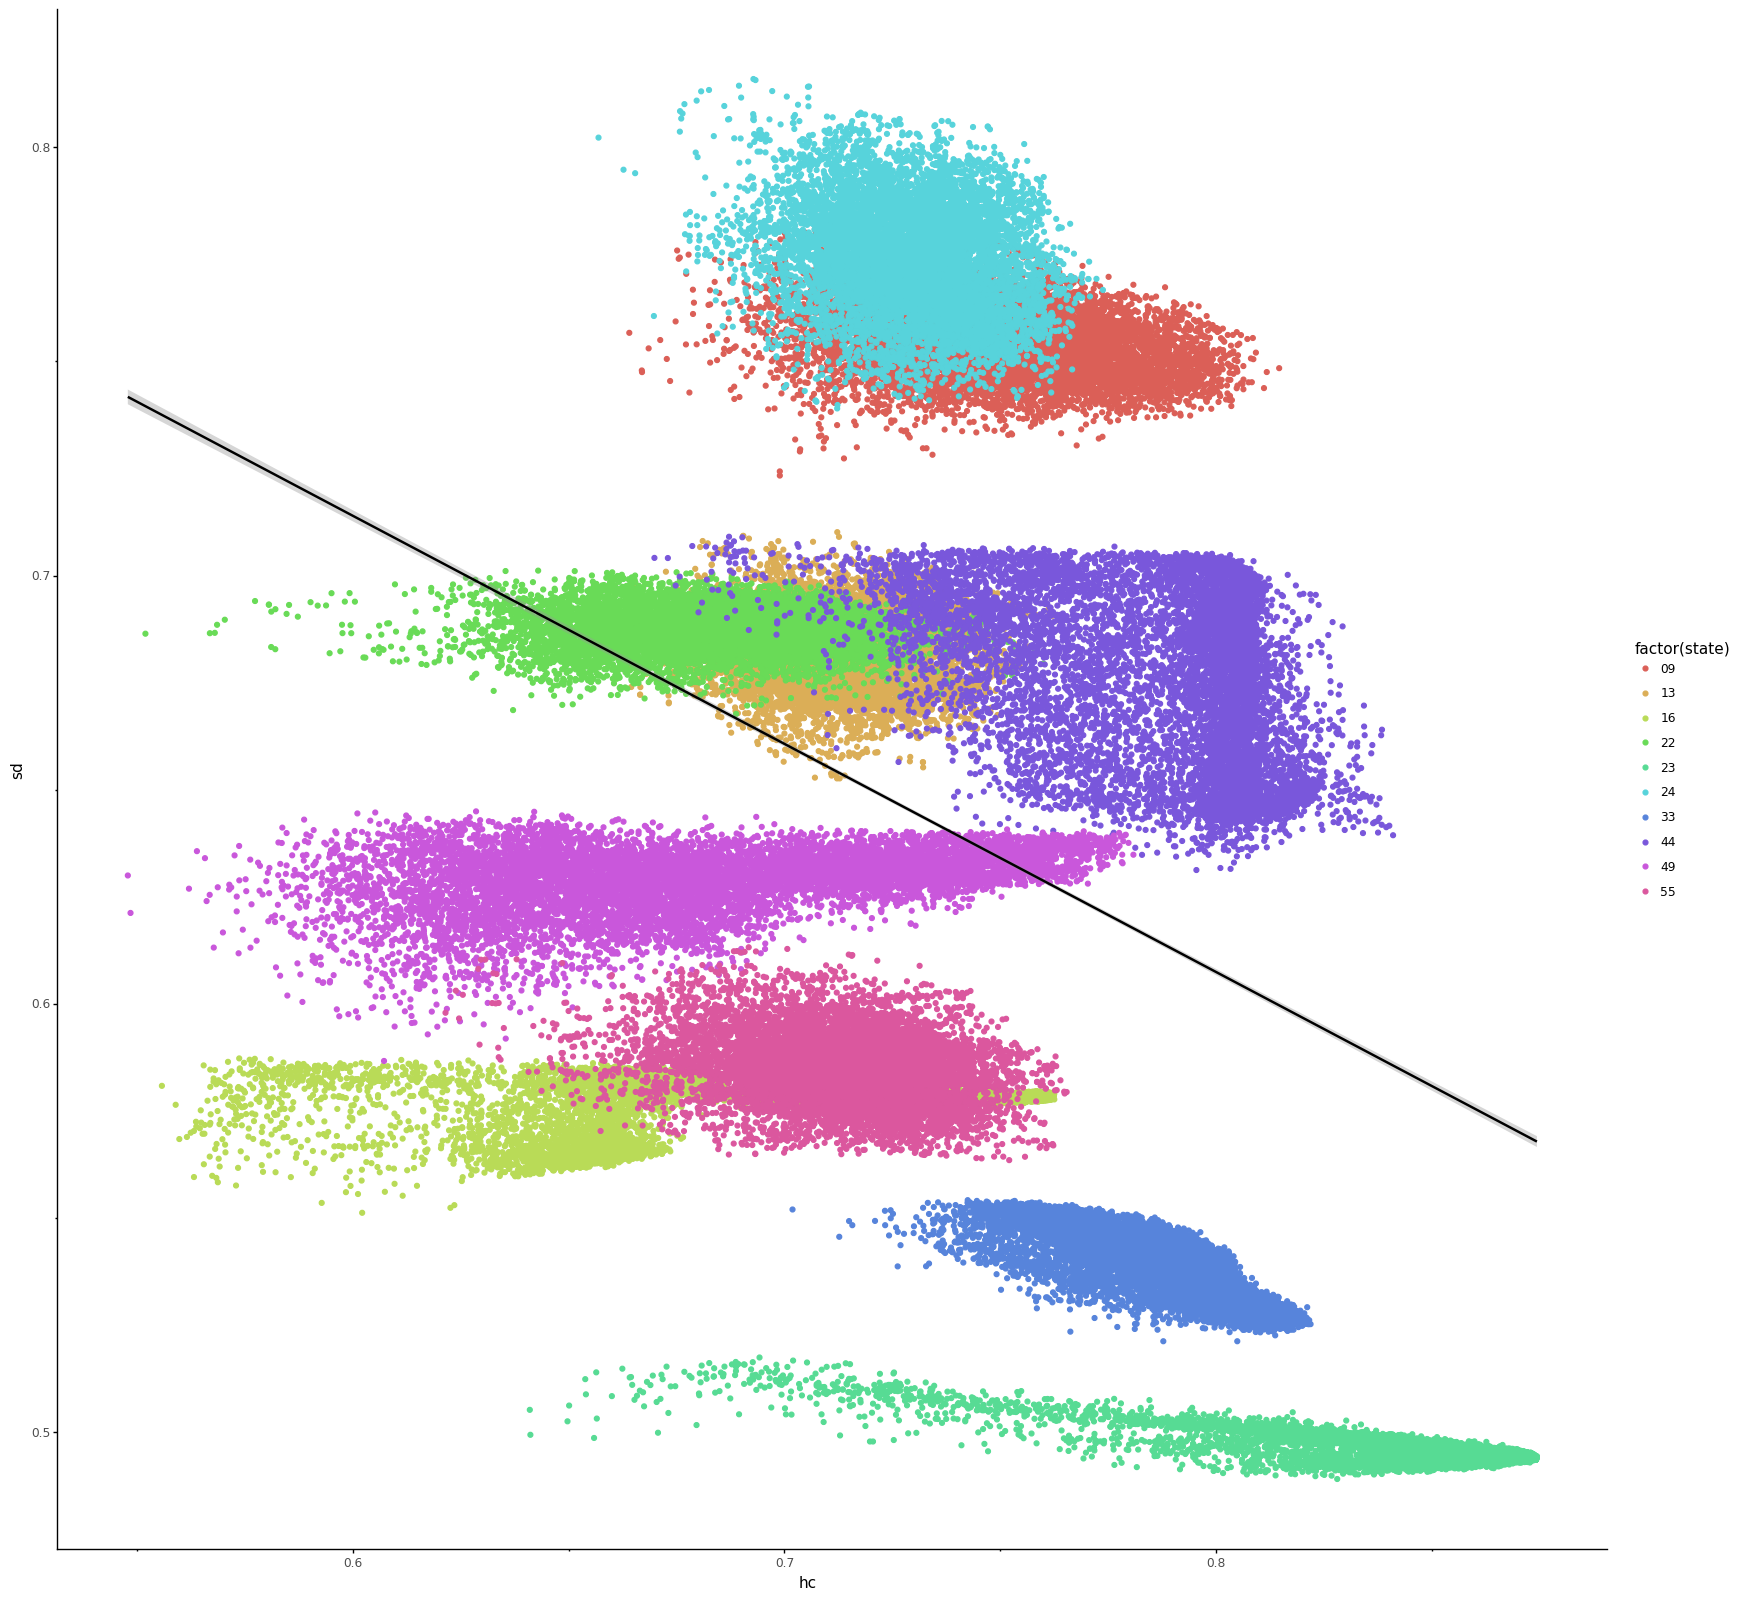
\includegraphics{../30_results/grouped_regressions.png}
\caption{Aggregating the individual states gives an inflated estimate of
the effect of compactness and commits the ecological fallacy
\label{grouped_reg}}
\end{figure}

We must therefore control for state when running the regression. Thus, I
run a multivariate regression with the functional form
\[SpatialDiversity = \beta_0 +
\beta_1 Compactness + \beta_2 State\] where \(State\) is a dummy
variable, taking care to avoid the dummy variable trap.

Table \ref{table:ols_sd_hc} gives the results for the OLS regressions,
which are also displayed in Figure \ref{regression_coefficients}.

\begin{figure}
\centering
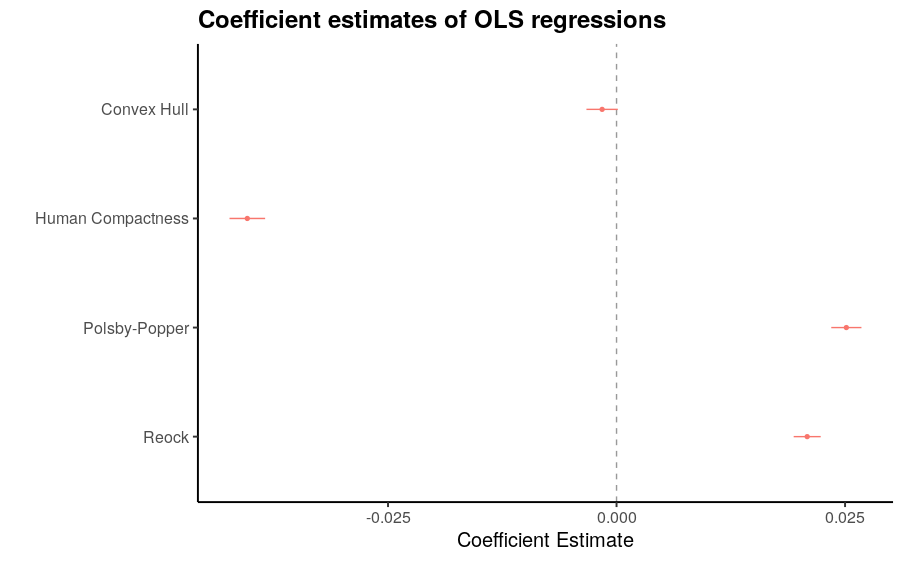
\includegraphics{../30_results/regression_coefficients.png}
\caption{\label{regression_coefficients}}
\end{figure}

I find that only human compactness has a statistically significant
negative coefficient on spatial diversity, while Polsby-Popper and Reock
have a significant positive effect on spatial diversity. This initial
result suggests two things: firstly, and rather disappointingly, that
optimising over the two most popular compactness measures may have
adverse effects on electoral competitiveness and responsiveness. More
encouragingly, though, these effects can be mitigated by the judicious
choice of compactness measure. The results show that optimising over
Convex Hull does not come at the cost of diversity, and that increasing
human compactness actually decreases spatial diversity.

\begin{table}[!htbp] \centering 
  \caption{OLS Regression of spatial diversity on various compactness metrics} 
  \label{table:ols_sd_hc} 
\begin{tabular}{@{\extracolsep{3pt}}lcccc} 
\\[-1.8ex]\hline 
\hline \\[-1.8ex] 
 & \multicolumn{4}{c}{\textit{Dependent variable:}} \\ 
\cline{2-5} 
\\[-1.8ex] & \multicolumn{4}{c}{Spatial diversity} \\ 
\\[-1.8ex] & (1) & (2) & (3) & (4)\\ 
\hline \\[-1.8ex] 
 Human compactness & $-$0.040$^{***}$ &  &  &  \\ 
  & (0.001) &  &  &  \\ 
  & & & & \\ 
 Polsby-Popper &  & 0.025$^{***}$ &  &  \\ 
  &  & (0.001) &  &  \\ 
  & & & & \\ 
 Reock &  &  & 0.021$^{***}$ &  \\ 
  &  &  & (0.001) &  \\ 
  & & & & \\ 
 Convex Hull &  &  &  & $-$0.002$^{*}$ \\ 
  &  &  &  & (0.001) \\ 
  & & & & \\ 
\hline \\[-1.8ex] 
Observations & 100,000 & 100,000 & 100,000 & 100,000 \\ 
State Dummies? & Yes & Yes & Yes & Yes \\ 
R$^{2}$ & 1.000 & 1.000 & 1.000 & 1.000 \\ 
Adjusted R$^{2}$ & 1.000 & 1.000 & 1.000 & 1.000 \\ 
Residual Std. Error (df = 99989) & 0.010 & 0.010 & 0.010 & 0.010 \\ 
F Statistic (df = 11; 99989) & 41,883,992$^{***}$ & 41,570,562$^{***}$ & 41,518,528$^{***}$ & 41,204,865$^{***}$ \\ 
\hline 
\hline \\[-1.8ex] 
\textit{Note:}  & \multicolumn{4}{r}{$^{*}$p$<$0.1; $^{**}$p$<$0.05; $^{***}$p$<$0.01} \\ 
\end{tabular} 
\end{table}

\hypertarget{robustness-check-1}{%
\paragraph{Robustness check}\label{robustness-check-1}}

\textsl{The results of the initial regression are suggestive, but not the last word. As
a robustness check, I run the same regression for for different subsets of the
generated plans, and find remarkably consistent results.}

\begin{center}\rule{0.5\linewidth}{\linethickness}\end{center}

The neutral ensemble algorithm I use to generate plans generates plans
that run the whole gamut of compactness scores, including both highly
compact plans and rather noncompact ones in the sample of 100,000. In
reality, however, legislators will try to optimise for compactness to
some degree. A plan proposed in real life---while not being optimally
compact---would be reasonably so. Rather than regressing over the entire
sample, then, we should specifically check the spatial diversity of
plans which exceed the threshold of ``reasonable compactness''.

But what is the threshold of ``reasonable compactness''? The choice of
the threshold cannot be determined \emph{a priori}. One would have to
know the distribution of compactness in a sample of plans generated in
real life. Of course, as real-life expert districtors do not produce a
distribution of plans, this is also a tall order. I therefore run the
same OLS regression for different thresholds of ``reasonable
compactness'', ranging from no cutoff (all plans) of plans to the top
10\% of plans\footnote{The results are similar when we take the top 5\%
  or 2\% of plans, but the small sample sizes of those thresholds mean
  that it is difficult to get statistical significance.}. That is to
say, I run the same OLS regression with smaller and smaller subsets of
the generated plans. The results are shown in Figure \ref{cutoffs}.

\begin{figure}
\centering
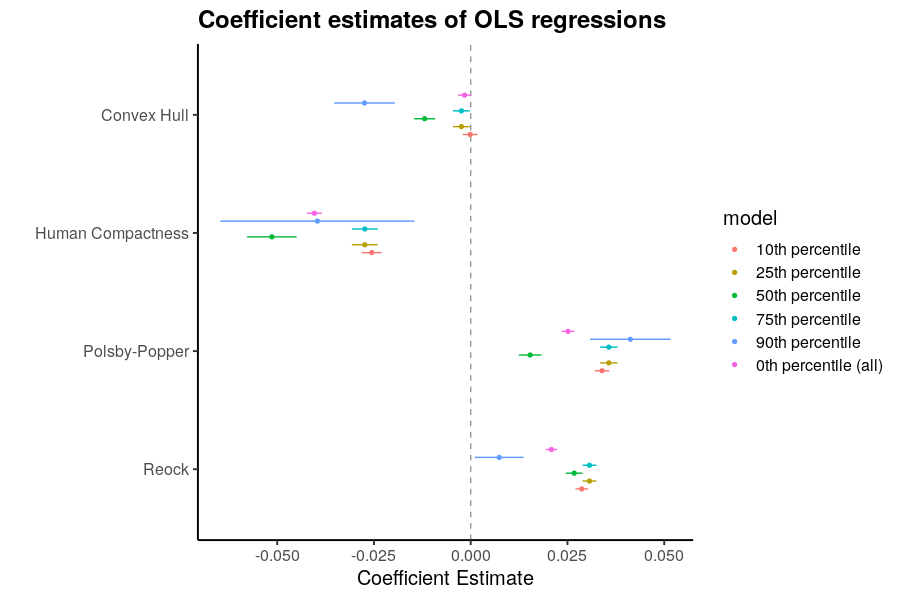
\includegraphics{../30_results/regression_coefficients_all.png}
\caption{OLS regression of spatial diversity on compactness for
different cutoffs \label{cutoffs}}
\end{figure}

While the results vary somewhat depending on our choice of threshold,
they are on the whole remarkably consistent. The Reock measure and
Polsby-Popper metrics perform poorly no matter what threshold one sets.
The Convex Hull metric is the best of the dispersion-based metrics. It
consistently has a negative coefficient, although the negative
coefficients are very small---particularly when the threshold is low.
Finally, the human compactness metric performs well on all subsamples.
The coefficient on human compactness is larger than all the other
metrics on all the thresholds---a strong indication that it is the
metric that best minimises spatial diversity.

\hypertarget{the-most-humanly-compact-plans-are-significantly-more-homogeneous-than-the-most-geometrically-compact-plans}{%
\subsubsection{The most humanly-compact plans are significantly more
homogeneous than the most geometrically-compact
plans}\label{the-most-humanly-compact-plans-are-significantly-more-homogeneous-than-the-most-geometrically-compact-plans}}

The OLS regressions we run give the relationship between compactness and
spatial diversity. But perhaps one is not concerned about the marginal
effect of compactness on diversity. One might ask a more basic question:
if we mandate that plans are ``reasonably compact''---whatever that
means---and force legislators to propose only plans that cross a
threshold of reasonable compactness, will that adversely affect spatial
diversity?

If there is indeed a fundamental trade-off between compactness and
spatial diversity, then we should observe the average spatial diversity
of highly compact plans to be higher than the spatial diversity across
all plans. I therefore compare the mean spatial diversity of top 500
plans under each compactness metric to the mean spatial diversity of all
plans. As a robustness check, I look at different proportions of top
plans (top 10\%/5\%/2\%) and obtain almost-identical results.
Encouragingly, there seems to be no trade-off between compactness and
spatial diversity: the mean spatial diversity in top compactness plans
is not higher than the overall mean spatial diversity. But only human
compactness has a mean spatial diversity \emph{significantly lower} than
the mean spatial diversity of all plans. In order to check the
significance of this result, I run a differences-in-means test using
Welch's t-test. I use Welch's t-test as Student's t-test relies on a
homogeneity in variances assumption. When the assumption of equal
variances is not met, Student's t-test yields unreliable results, while
Welch's t-test controls Type 1 error rates as expected
\citep{delacre2017}. In this case, since the top plans come from
different distributions, it is unlikely that the variances are
homogeneous. Only human compactness had a statistically significant
difference in mean spatial diversity. For completeness, I also ran
pairwise differences-in-means tests between all four metrics, for a
total of 6 tests. The results are as follows:

The results are shown in Figure \ref{diff_in_means}.

\begin{figure}
\centering
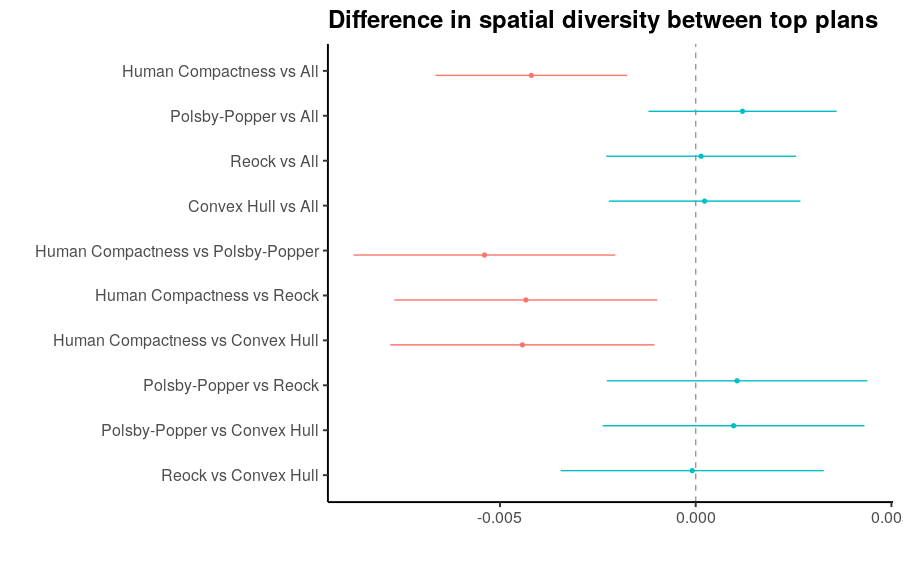
\includegraphics{../30_results/diff_in_means.png}
\caption{Mean spatial diversity of top plans under each compactness
measure \label{diff_in_means}}
\end{figure}

As expected, there were no significant differences in means between any
of the geometric compactness metrics, but there was a significant
difference in the means between human compactness and the other
compactness metrics. The results show that the top plans under human
compactness have significantly lower spatial diversity than the top
plans under other compactness metrics.

\hypertarget{robustness-check-2}{%
\paragraph{Robustness check}\label{robustness-check-2}}

\textsl{As a robustness check, and to prevent committing the ecological fallacy
(drawing inferences about individual-level differences from aggregate-level
data), I run 40 individual t-tests to check if there are differences in spatial
diversity on a state-by-state level. The top plans under human compactness are
more likely to be significantly more homogeneous than top plans under other
compactness metrics.}

\begin{center}\rule{0.5\linewidth}{\linethickness}\end{center}

While this analysis is suggestive, there are two rejoinders to this.
Firstly, one could argue that the difference in means is quite small:
only 1.5\% of the total variance in spatial diversity. Secondly, one
might think that looking only at the aggregated results could be
misleading. A difference in means in the aggregate could be due to one
or a few outlier states driving the results.

To address these two criticisms, I run Welch's t-tests for each metric
for all ten states (giving a total of 40 t-tests). The full list of
t-tests is available in Appendix B. Once again, human compactness
performs the best. The top plans under the Reock metric have
statistically significant negative differences in spatial diversity
means in 3 out of 10 states. Polsby-Popper and Convex Hull do a little
better with 4 out of 10 states. Human Compactness outperforms with a
total of seven states. If we look at \emph{meaningful} differences---not
just statistically significant ones (instances where the mean is lower
by more than 5\% of the total variance)---then human compactness
outperforms by a wide margin. Human compactness has a statistically
significant and meaningfully lower spatial diversity in six of the
states. Reock does in two states, and Convex Hull and Polsby-Popper only
in one. Finally, in two cases (both under the human compactness metric),
the difference is so meaningful that it makes up 25\% and 35\% of the
total variance. Concretely, the spatial diversity of all 10,000 New
Hampshire plans lie within a range of 0.03. The top 1,000 plans under
human compactness have a spatial diversity that is 0.01 lower than the
mean --- a very meaningful effect that spans one-third of the total
range. Far from being a small effect, it seems that the choice of
compactness metric to optimise over can have very meaningful impacts.

What do the difference in means actually imply in terms of proposed
plans? Table \ref{table:top_plans_sd_percentile} shows what percentile
the top 10 percent of plans under each metric would occupy in the
distribution of 10,000 plans (lower is better). If there is no
relationship between a compactness metric and spatial diversity, then we
should expect the mean percentile to lie around 50 percent. If, however,
the top plans under a metric are significantly less spatially diverse,
then we should see a low percentile for many of the states. In the
table, I have \textbf{bolded} the best-performing metric in each row,
subject to it being less than the median (\textless{}50th percentile).
As before, I run robustness checks and get qualitatively similar results
for various threshold cut-offs.

\begin{table}[h!]
\begin{center}
\caption{What percentile the top 10 percent of plans under each metric occupy (lower is better)}
\label{table:top_plans_sd_percentile}
\begin{tabular}{@{\extracolsep{3pt}}lrrrr} 
\toprule
{} &     hc &     pp &  reock &     ch \\
\midrule
0 Connecticut &  \textbf{34.31} &  54.02 &  55.61 &  48.25 \\
1 Georgia &  48.29 &  \textbf{44.24} &  48.34 &  47.62 \\
2 Idaho &  59.92 &  48.62 &  \textbf{20.90} &  26.88 \\
3 Louisiana &  \textbf{39.03} &  39.12 &  42.45 &  41.24 \\
4 Maine &  26.22 &  92.48 &  78.12 &  \textbf{23.56} \\
5 Rhode Island &  \textbf{23.32} &  56.46 &  53.71 &  52.70 \\
6 Maryland &  36.99 &  \textbf{33.00} &  \textbf{33.00} &  48.68 \\
7 New Hampshire &   \textbf{8.25} &  58.08 &  40.30 &  65.73 \\
8 Utah &  77.05 &  61.72 &  58.57 &  59.92 \\
9 Wisconsin &  \textbf{34.09} &  42.14 &  47.26 &  43.07 \\
\bottomrule
Mean percentile & \textbf{38.75} &  52.99  &  47.83 &  45.77 \\
\bottomrule
\end{tabular}
\end{center}
\end{table}

The table shows that the human compactness metric consistently
outperforms the other metrics in many of the states, forestalling the
criticism that the results may be driven by one or two outliers. While
human compactness does particularly well in New Hampshire and Rhode
Island, it still performs best overall even if we remove those two
states from consideration.

\hypertarget{discussion}{%
\section{Discussion}\label{discussion}}

\hypertarget{i-found-no-consistent-trade-off-between-compactness-and-communities-of-interest}{%
\subsection{I found no consistent trade-off between compactness and
communities of
interest}\label{i-found-no-consistent-trade-off-between-compactness-and-communities-of-interest}}

Is there a fundamental trade-off between compactness and communities of
interest, as proxied by district homogeneity? The answer seems to be: it
depends on how you measure compactness. For geometric compactness
measures, the results are equivocal: OLS regressions indicate that there
is some trade-off between compactness and homogeneity, while
difference-in-means tests indicate no such trade-off. Point-based
distance metrics seem to fare better. In fact the results show that
rather than a trade-off, there is a synergy between human compactness
and district homogeneity.

It was the right call to use many different compactness metrics, due to
the frequency at which even very similar compactness measures disagree.
The Maine entry in Table \ref{table:top_plans_sd_percentile} is a good
example. The top Polsby-Popper plans lie in the 92nd percentile of all
plans---shockingly high---but looking at the Reock and Convex Hull
measures paint a much less one-sided picture. In fact, it is surprising
that the Reock and Convex Hull percentiles differ so radically, seeing
as the measures differ only in the bounding shape (convex polygon versus
a circle) of the district.

If we had used only the Polsby-Popper metric in our analyses, we would
have (erroneously) concluded that Maine's political geography was
fundamentally incompatible with compactness. This casts doubt upon work
that uses only a singular compactness metric to score districting plans.
Without wishing to single out any work in particular (many other papers
do the same thing), \cite{s2020} uses only the Polsby-Popper measure to
analyse only two states. My data suggest that this analysis is
insufficient---severely curtailing the generalisability of the work.

\hypertarget{human-compactness-seems-to-best-encompass-communities-of-interest}{%
\subsection{Human compactness seems to best encompass communities of
interest}\label{human-compactness-seems-to-best-encompass-communities-of-interest}}

{[}TODO -- reword to talk about communities of interest/homogeneity{]}

Does spatial diversity give us a good reason to choose one compactness
metric over another? Yes. The data show that human compactness better
tracks spatial diversity, which in turn correlates with democratic
outcomes like participation, responsiveness and competitiveness. This
finding consistently repeats itself throughout different analyses,
different thresholds, and different aggregation functions. The
implication is clear: if we believe Stephanopoulos's work on the
benefits of lower spatial diversity, then adopting human compactness
will give us better plans.

To be fair, there are many other considerations that go into choosing a
compactness metric, and I have alluded to several in the previous
sections. First is objectivity. Geometric compactness measures were
invented in the first place---almost six decades ago---to measure and
prosecute gerrymandering objectively: ``{[}compactness{]} remains
subjective in that no method of measurement has gained general
acceptance'' \citep[p.~74]{reock1961}.

But second---and possibly far more important---is explainability.
Compactness metrics feature prominently in spheres outside academic
political science, from general political discourse to amicus briefs for
the Supreme Court. The seminal work by Reock almost sixty years ago says
``the best use for the method of measuring compactness outlined here is
\emph{as a tool for the courts and as a weapon for public opinion}''. It
is thus incredibly important that a compactness metric be intuitive and
explainable to laymen. This almost entirely rules out overly
mathematical measures like \cite{dc2016} that use graph theory and
minimise cut edges, or uninterpretable measures like \cite{kingwp} that
build a ``black box'' machine learning model.

While geometric compactness metrics are simple enough to explain, they
lack a normative appeal. It is almost too easy to criticise geometric
compactness metrics on the basis of irrelevance. If we ask: \emph{why}
should districts follow some regular shape? the answer is not
immediately forthcoming, and in fact many have pointed out correctly
that there is little reason to do so \emph{eo ipso}.

Human compactness seems to meet both these criteria. It encapsulates the
notion of ``communities of interest'', while sidestepping the problem of
having to define, delineate and make subjective judgement calls on these
communities. And while it's not obvious that districts should conform to
some regular polygon, the idea of putting people who live together in
the same voting district has a strong normative force with great
intuitive appeal. Finally, the lower (but still substantially positive)
correlation between human compactness and the other compactness measures
suggests that human compactness qualitatively differs from geometric
compactness.

\hypertarget{directions-for-future-work}{%
\subsection{Directions for future
work}\label{directions-for-future-work}}

Future work should look at expanding the scope of the analysis in three
ways: the number of states, the number of compactness measures, and the
number of outcomes of interest.

My work analyses 10 out of the 50 states. Restricting analysis to a
subset of states is common in other redistricting work, due to the
onerous computational burdens of the procedure. \cite{ddj2019comp}
measure the effect of competitiveness on partisanship for five states,
and \cite{s2020} looks at the trade-off between compactness and partisan
symmetry for only two states. We know, however, that this has
implications on external validity. While my analysis covers more states
than much of the literature, further work should nonetheless extend the
analysis to cover more states---especially large states like Texas,
Florida and California. Future work should also analyse more compactness
measures. Of particular interest would be other point-wise distance
metrics like bizarreness, and \citeauthor{kingwp}'s (\citeyear{kingwp})
metric that attempts to imitate human perception.

Finally, future work should analyse a variety of other outcomes of
interest apart from spatial diversity. As the primary draw of
point-based distance measures is that it should keep communities of
people together in the same district, I would particularly like to see
future work whether human compactness does a better job of keeping
communities of interest together. We should also examine the effect of
compactness on a wider range of normative outcomes---not just procedural
ones. Districting affects many other things: political knowledge,
turnout, and federal spending \citep{snyder2010}, but work so far has
been focused almost entirely on electoral competitiveness.

\hypertarget{conclusion}{%
\subsection{Conclusion}\label{conclusion}}

{[}TODO{]}

\hypertarget{acknowledgements}{%
\subsection{Acknowledgements}\label{acknowledgements}}

\begin{itemize}
\tightlist
\item
  Big thanks to Bassel;
\item
  Big thanks to Daryl Deford, for explaining MCMC, Gerrychain, and
  generating the districting plans;
\item
  and Filip, for walking through with me all my ideas from May 2019
  until now;
\item
  and Stephanopoulos, for giving me his spatial diversity data;
\item
  Eubank and Rodden, for being kind enough to respond to my emails, and
  their VRP data,
\item
  Tak Huen, for giving me copies of \emph{Political Analysis}, from
  which the initial idea of this thesis came;
\item
  Zun Yuan, for letting me bounce optimisation ideas off him;
\item
  Sergi, for being the tutor that got me interested in Politics;
\item
  Am I allowed to thank Andy or name him as my supervisor? Ask Tak Huen
  about this
\end{itemize}

Images of Reock and PP metric taken from
\href{https://fisherzachary.github.io/public/r-output.html}{fisherzachary.github.io}

\pagebreak{}

\hypertarget{technical-appendix-a-evaluating-different-methods-of-plan-generation}{%
\section{Technical Appendix A: evaluating different methods of plan
generation}\label{technical-appendix-a-evaluating-different-methods-of-plan-generation}}

The idea of drawing a large number of districting plans with a computer
has a long and storied history, starting in the 60s and 70s. The
approach has almost always been used to identify gerrymandering; for
instance \cite{ccd2000} build an algorithm to ``quantitatively
{[}assess{]} whether the {[}1990 South Carolina{]} plan is a racial
gerrymander''. More recently, \cite{cr2013} ``generat{[}e{]} a large
number of hypothetical alternative districting plans that are blind as
to party and race, relying only on criteria of geographic contiguity and
compactness.'' They do this using a Markov Chain simulation algorithm, a
procedure that makes iterative changes for a large number of steps until
a unique districting plan emerges. At each step of
\citeauthor{ccd2000}'s algorithm, they randomly select a Census Block
Group to serve as a ``seed'' of the district, then randomly add its
neighbouring block groups to it until a district with the desired
population is formed. Similarly, \citeauthor{cr2013} begin by
initialising all voting precincts as an individual, separate district,
then randomly agglomerating neighbouring precincts until the desired
number of districts is reached.

While this standard iterative algorithm enjoys a certain degree of
success, it has one crippling weakness. The way in which this class of
algorithms operates necessarily explores only a tiny subset of all
possible districting plans. Subsequent work pointed out this flaw:
\citeauthor{mm2018} wrote that automated processes ``may take a biased
sample of all possible legislative maps\ldots{} and fail to efficiently
produce a meaningful distribution of all alternative maps''. And
\citeauthor{fifieldwp} contend that ``{[}standard Monte Carlo
algorithms{]} are unlikely to yield a representative sample of
redistricting plans for a target population.'' \footnote{See
  \cite{fifieldwp}, pg. 16, for a technical explanation of why these
  algorithms don't produce uniform redistricting plans: ``For example
  \ldots{}, the creation of earlier districts may make it impossible to
  yield contiguous districts. These algorithms rely on rejection
  sampling to incorporate constraints, which is an inefficient strategy.
  More importantly, the algorithms come with no theoretical result and
  are not even designed to uniformly sample redistricting plans.''} This
poses a huge issue for the validity of any statistical analysis, because
any correlation that we discover on a biased subset of plans may be
spurious when measured over the actual distribution of plans. \footnote{Generating
  a biased sample is not necessarily a problem if all you want to do is
  \emph{optimise}, e.g.~draw the most compact plan possible. Recent work
  builds upon this standard algorithm, using Voronoi diagrams or
  iterative flood fill procedures rather than random chance, to assign
  the precincts to be agglomerated. See \cite{lf2019} for a technical
  overview.}

\hypertarget{markov-chain-algorithms}{%
\paragraph{Markov Chain algorithms}\label{markov-chain-algorithms}}

Thankfully, scholars have developed an improvement over the standard
algorithm with stronger theoretical guarantees. This second class of
algorithms reframe the districting problem as a \emph{graph partition}
problem (borrowing insights from graph theory and computer science), and
use a \emph{Markov Chain Monte Carlo} (MCMC) approach to sample possible
districting plans. This approach is best laid out in \cite{fifieldwp}.
The approach first initialises a specific graph partition. A graph
partition is an assignment of Census Tracts/Blocks to districts ---
basically a districting plan. This is the first step of the Markov
Chain. Then it \emph{flips} a random node of the graph to get another
valid partition. This process is repeated until the Markov Chain
approaches its steady state distribution: when this happens, the Markov
chain is called ``well-mixed''.

This class of algorithms inherit desirable well-known theoretical
guarantees of the Markov Chain.\footnote{See \cite{ddj2019recom} for a
  technical overview.} They are therefore much less likely (both
theoretically and empirically) to generate a biased subset of plans.
Conducting a small-scale validation study on a 25-precinct set,
\citeauthor{fifieldwp} compare the distribution of plans generated by
their algorithm to those generated by the standard redistricting
algorithm. They prove that their algorithm produces plans that hew much
more closely to the \emph{actual} distribution of all possible
districting plans.

Due to the many advantages of the MCMC approach, I use it in all my
analyses. However, there are many ways to conduct an MCMC analysis. The
key question is how one should sample from the near-infinite pool of
possible plans. State-of-the-art literature in this space use one of
three main approaches, all of which have their pros and cons.

The first is to get a sense for the properties of extremely compact
plans under each compactness measure by using a local optimization
technique, starting at a whole bunch of different initial seeds using
the single node \texttt{Flip} proposal. This approach gives us the most
compact plans, and is often used to find the ``maximal'' or ``best''
districting plans. However, it will---by design---only explore a very
tiny subset of all plausible districting plans. Also, because the
\texttt{Flip} proposal is very state-dependent, the initial state can
affect the results greatly.

The second is a middle-of-the-road approach, using a global proposal
distribution and a Metropolis-Hasting acceptance function to sample from
a distribution over plans that is proportional to
\(e^{(-\beta \times Compactness)}\). This will give us a distribution of
plans that is biased towards compact ones, but also contains some
noncompact plans.

One can get different distributions of plans depending on the specific
acceptance (score) function. For instance, \cite{dd2019va} prioritises
plans that have fewer locality splits and/or sustain a Black
majority-minority district. \cite{h2018} use a complicated score
function that takes into account county splitting, population deviation,
compactness and minority representation. If I were to use this approach,
I would define four different score functions corresponding to the
different compactness measures, and compare the resulting distributions
that result from each measure.

Finally, one can sample from a distribution that doesn't incorporate any
compactness score at all and extract the plans that achieve a good score
under each metric. This approach is used in \cite{ddj2019comp}, where
they generate a large neutral ensemble of districting plans and then
subsequently filter the plans according to increasingly strict vote-band
constraints. The advantage of this approach is that it casts the widest
net: all plausible districts (subject to the equal population bound) are
explored. The disadvantage is that the odds of sampling an `optimal'
district are incredibly low, which makes it suboptimal for algorithms
that aim to build the ``best'' plan.

\hypertarget{choosing-the-best-mcmc-approach}{%
\paragraph{Choosing the best MCMC
approach}\label{choosing-the-best-mcmc-approach}}

To recap, there are three plausible MCMC approaches to generate a large
subset of redistricting plans: local optimisation, score function, or
neutral ensemble. I examine them each in turn and decide on the neutral
ensemble approach because it generates the largest and most
representative subset of redistricting plans, which best represents the
plans that legislators are likely to draw in real life.

The first proposal is local optimisation. Local optimisation approaches
like the \texttt{Flip} proposal have one key problem. The ``mixing
time'' of the Markov Chain under the \texttt{Flip} proposal---that is,
the number of steps it takes for the Markov Chain to be ``close enough''
to the stationary distribution---is very large. What that means is that
the \texttt{Flip} proposal tends to generate very uncompact, snakelike
districts in the beginning, as can be seen in Figure
\ref{recom_vs_flip}. It will take millions of steps for plans under the
\texttt{Flip} proposal to reach a satisfactory districting plan. As
such, I prefer the Recombination (Recom) distribution by
\citeauthor{ddj2019recom}, which uses a spanning tree method to
bipartition pairs of adjacent districts at each step
\citep{ddj2019comp}. This proposal distribution improves upon the
\texttt{Flip} proposal by decreasing the mixing time needed to reach a
satisfactory districting plan.

\begin{figure}
\centering
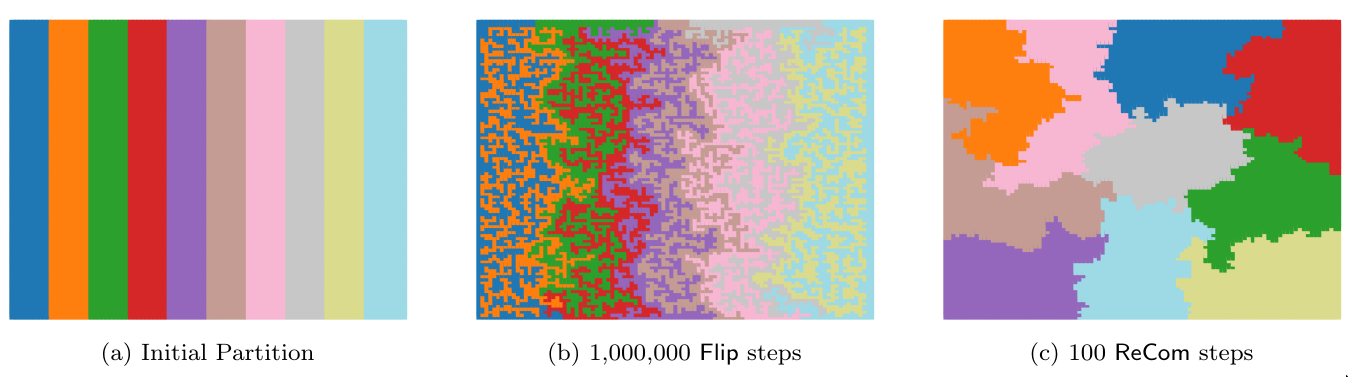
\includegraphics{img/recom_vs_flip.png}
\caption{\label{recom_vs_flip} The \texttt{Recom} proposal generates
more realistic plans in much fewer steps. Taken from
\cite{ddj2019recom}.}
\end{figure}

Mixing time aside, the extreme compactness of local optimisation is in
fact something that I want to avoid. I aim to find out if mandating
compactness in state constitutions can inadvertently adversely affect
democratic representation. But restricting one's analysis to extremely
compact plans means that we cannot say much about the relationship
between compactness and spatial diversity. In addition, extremely
compact plans are \emph{not} a representative subset of the plans
unbiased redistrictors might draw. This is because redistrictors care
about a lot of other considerations apart from compactness, and
therefore most definitely do not optimise solely over compactness. State
constitutions demand that plans be ``reasonably compact'', not
``maximally compact'': it's vanishingly unlikely that those extremely
compact plans would resemble the types of plans that would be drawn in
real life. As such, \emph{even} if I found that optimally compact plans
had greater spatial diversity, this would have very little bearing on
redistricting policy. It's far more instructive to see whether the
relationship holds in the plans that legislators could actually be
expected to draw.

\begin{center}\rule{0.5\linewidth}{\linethickness}\end{center}

How can we get a representative subset of plans that legislators could
actually be expected to draw? Given that legislators care a lot about
many different considerations, might it be better to try and include
these considerations into the score function? This is what the second
approach does. While this approach holds strong theoretical merit, I
find that this approach introduces too many degrees of freedom. The
choice of what factors to include in the score function is contentious:
\citeauthor{h2018} use population deviation, Polsby-Popper score, county
boundaries and minority deviation. But they could just as easily have
included factors such as proportionality or number of cut edges
(proposed in \cite{dc2016}) for instance. Even if there is a strong
justification for including exactly those factors, there is still
significant researcher freedom to operationalise the scores. For
instance, \citeauthor{h2018} and \citeauthor{dd2019va} both include a
population deviation score, but operationalise the metric differently.

Furthermore, any score function has to be assigned specific weights---
but this assignment is somewhat arbitrary and open to argument. For
instance, \citeauthor{h2018} ``chose a VRA score function which awards
lower scores to districting plans which had one district close to
44.48\% African-Americans and a second district close to 36.20\%
African-Americans'', on the basis that the 2016 districting plan which
was accepted by the Court had districts with those proportions. But this
is incredibly arbitrary. Obviously, just because a particular district
was accepted by the Court with those proportions of African-Americans
doesn't imply that those exact proportions of African-Americans are
optimal.

To be clear, these problems are not insurmountable. If there is a strong
theoretical basis for one particular operationalisation over another,
then the criticism of researcher fiat largely loses its bite.
Furthermore, the results obtained are robust to a variety of
perturbations. \cite{h2018} change the weights and threshold values as a
robustness check and find qualitatively similar results. Nonetheless,
different results can occur. And if two different operationalisations or
factor weights yield qualitatively different results, how would we
adjudicate between them? For these reasons, I choose not to use the
second approach.

\begin{center}\rule{0.5\linewidth}{\linethickness}\end{center}

Finally, the neutral ensemble approach is the most permissive, and thus
gives us the best chance of getting a representative sample of
legislators' plans. It generates a neutral ensemble and does not favour
one plan over another (except for some minimal compactness and
population deviation requirements). This approach gives us the largest
space of plausible plans, which has a key advantage: it allows the
results to be applicable even for districting algorithms that do not use
an MCMC approach. This includes not only the regular low-tech way of
drawing districts, but also other automated districting algorithms like
\cite{mm2018} and \cite{lf2019}.

Therefore, I elect to use the last, ``neutral walk'' approach. I use a
global \texttt{Recom} proposal to generate the states, but accept every
proposal subject to minimal population deviation requirements. This
gives me a neutral ensemble of 10,000 plans for every state.

\hypertarget{technical-appendix-b-optimisations-used-in-computing-the-human-compactness-metric}{%
\section{Technical Appendix B: Optimisations used in computing the human
compactness
metric}\label{technical-appendix-b-optimisations-used-in-computing-the-human-compactness-metric}}

Maybe not necessary, but talk about the precomputation steps and saving
the pointwise distances

\hypertarget{appendix-a}{%
\section{Appendix A:}\label{appendix-a}}

\hypertarget{appendix-b-results-of-difference-in-means-tests-for-individual-states}{%
\section{Appendix B: Results of difference-in-means tests for individual
states}\label{appendix-b-results-of-difference-in-means-tests-for-individual-states}}

Here I compare the average spatial diversity of all 10,000 plans per
state to the average spatial diversity of the 500 most compact plans per
state.

I present the results for each state and each metric in the ensemble,
using Welch's t-test.

\begin{tabular}{lrlrrrrr}
\toprule
{} &  state & metric &  mean\_diff &  variance &  pct\_variance &      t-stat &        p-value \\
\midrule
0  &      0 &     hc &  -0.003460 &  0.058642 &     -5.900607 &  -17.425785 &   1.366961e-61 \\
1  &      0 &     pp &   0.000069 &  0.058642 &      0.118009 &    0.288166 &   7.732681e-01 \\
2  &      0 &  reock &   0.000381 &  0.058642 &      0.650317 &    1.624462 &   1.045297e-01 \\
3  &      0 &     ch &  -0.001042 &  0.058642 &     -1.776135 &   -5.014481 &   6.033771e-07 \\
4  &      1 &     hc &  -0.000513 &  0.057499 &     -0.892208 &   -1.868482 &   6.193359e-02 \\
5  &      1 &     pp &  -0.001423 &  0.057499 &     -2.475505 &   -4.986335 &   7.054193e-07 \\
6  &      1 &  reock &  -0.000498 &  0.057499 &     -0.865298 &   -1.692770 &   9.076060e-02 \\
7  &      1 &     ch &  -0.000678 &  0.057499 &     -1.178930 &   -2.231754 &   2.581874e-02 \\
8  &      2 &     hc &   0.001489 &  0.036047 &      4.131827 &   26.809567 &  2.038788e-153 \\
9  &      2 &     pp &   0.001104 &  0.036047 &      3.062205 &   10.321991 &   2.820313e-24 \\
10 &      2 &  reock &  -0.000188 &  0.036047 &     -0.520417 &   -0.859779 &   3.900941e-01 \\
11 &      2 &     ch &   0.000383 &  0.036047 &      1.063637 &    2.841225 &   4.560090e-03 \\
12 &      3 &     hc &  -0.001257 &  0.033457 &     -3.756204 &   -9.240446 &   9.523388e-20 \\
13 &      3 &     pp &  -0.001245 &  0.033457 &     -3.720159 &   -7.632057 &   4.670461e-14 \\
14 &      3 &  reock &  -0.000776 &  0.033457 &     -2.318159 &   -5.132091 &   3.320205e-07 \\
15 &      3 &     ch &  -0.000927 &  0.033457 &     -2.770633 &   -7.108140 &   1.896994e-12 \\
16 &      4 &     hc &  -0.001902 &  0.028376 &     -6.704063 &  -49.155427 &   0.000000e+00 \\
17 &      4 &     pp &   0.005131 &  0.028376 &     18.081320 &   38.153281 &  1.090249e-206 \\
18 &      4 &  reock &   0.001304 &  0.028376 &      4.596054 &   20.334160 &   7.714653e-84 \\
19 &      4 &     ch &  -0.002035 &  0.028376 &     -7.171113 &  -50.341694 &   0.000000e+00 \\
20 &      5 &     hc &  -0.019707 &  0.077819 &    -25.324736 &  -43.785027 &  7.817121e-271 \\
21 &      5 &     pp &   0.007385 &  0.077819 &      9.490310 &   14.029691 &   8.033314e-42 \\
22 &      5 &  reock &   0.005601 &  0.077819 &      7.197869 &   10.059549 &   5.666063e-23 \\
23 &      5 &     ch &   0.004848 &  0.077819 &      6.229592 &    8.615116 &   2.011837e-17 \\
24 &      6 &     hc &  -0.004913 &  0.076917 &     -6.386934 &  -12.541515 &   4.676097e-34 \\
25 &      6 &     pp &  -0.006333 &  0.076917 &     -8.233653 &  -16.445177 &   3.655560e-55 \\
26 &      6 &  reock &  -0.006334 &  0.076917 &     -8.235342 &  -17.317992 &   1.527167e-60 \\
27 &      6 &     ch &  -0.000795 &  0.076917 &     -1.033852 &   -1.809545 &   7.061978e-02 \\
28 &      7 &     hc &  -0.011556 &  0.032940 &    -35.083239 & -120.004988 &   0.000000e+00 \\
29 &      7 &     pp &   0.002150 &  0.032940 &      6.527335 &    9.218455 &   1.208411e-19 \\
30 &      7 &  reock &  -0.002165 &  0.032940 &     -6.573630 &  -11.615082 &   6.541658e-30 \\
31 &      7 &     ch &   0.004050 &  0.032940 &     12.294876 &   17.193270 &   1.023553e-59 \\
32 &      8 &     hc &   0.005538 &  0.058276 &      9.503582 &   42.778404 &  4.401068e-291 \\
33 &      8 &     pp &   0.002962 &  0.058276 &      5.082034 &   18.477814 &   2.578165e-69 \\
34 &      8 &  reock &   0.002492 &  0.058276 &      4.275665 &   14.864941 &   8.132217e-47 \\
35 &      8 &     ch &   0.002689 &  0.058276 &      4.613737 &   16.787183 &   1.984654e-58 \\
36 &      9 &     hc &  -0.003290 &  0.049699 &     -6.619743 &  -13.092609 &   8.687410e-37 \\
37 &      9 &     pp &  -0.001645 &  0.049699 &     -3.309711 &   -6.053633 &   1.889349e-09 \\
38 &      9 &  reock &  -0.000677 &  0.049699 &     -1.361577 &   -2.476624 &   1.340008e-02 \\
39 &      9 &     ch &  -0.001482 &  0.049699 &     -2.982079 &   -5.561983 &   3.278783e-08 \\
\bottomrule
\end{tabular}

\clearpage

\bibliography{references.bib}

\end{document}
